\chapter{Experiments using the magnetometer\label{ch:results}}

In this Chapter, I present the main results on measurements of the
properties of the magnetometer, optimization studies, and applications
of the magnetometer to characterize magnetic fields.  The main studies
that are presented are:
\begin{itemize}
\item Measurements of magnetic fields over long timescales using FID mode.
%  Conclusion: fields drift over time.  Question: how much is due to
%  magnetometer drift vs. other sources?
\item Adjustment of the pump and probe timescales in order to measure
  the field faster.
%  Allowed us to measure faster.
\item Magnetometer drift compared with drifts in the coil current and
  room temperature.  This study aimed at finding sources of drifts.
%Conclusion: neither drift seems
%  particularly correlated with field drift over long time periods.
%  Temperature stability seems quite good, consistent with Michi's
%  thesis.  Side conclusion: when field {\bf only} is changed, the
%  magnetometer responds as expected.  Implies that magnetometer works
%  well at sensing small changes in field, at least on shorter
%  timescales.
\item Studies of degaussing, which in part tell the story of our
  degaussing development and learning.  This includes studies of:
%with multiple goals, telling the story of
%  our degaussing
  \begin{itemize}
    \item the degaussing setup and testing it near zero field
%we set up the
%      system, we tested mainly sample rate (related to number of
%      oscillations) stated to be important in Thiel et al.  We found
%      that if the innermost shield was already degaussed that
%      additional poor/rapid degauss did not screw it up as badly as we
%      expected, until degaussing was very rapid.
    \item initial operations at non-zero field, and
%Ramp field to large values, without
%      degaussing was bad.  After degaussing was better.
    \item final degaussing procedure, in which degaussing the next to
      innermost shield was studied.
  \end{itemize}
\item Studies of laser locking and tuning, and the requirements on
  tune stability
%again multiple goals:
%  \begin{itemize}
%    \item Lock point or laser seems to drift over time.  See ``Drift
%      is about 120 pT'' where statistical error gets worse.  Also
%      would lose lock sometimes.  We think this may be due to PBS.
%    \item Other concern is whether drift of lock affects measured
%      field.  Studied by ``manual locking'' and found not to be
%      important.  Lock drift does not affect measured field drift very
%      much, but does affect statistical precision of magnetometer.
%  \end{itemize}
\item Studies pushing below 1~pT in an individual FID measurement.
  This includes adjustment of the pump and probe powers, and lock-in
  amplifier settings.  As will be shown, this study revealed problems
  in the procedures used to determine the precession frequency at such
  high precision and suggests avenues for further study.
%But when
%  we improved the statistical precision significantly, we began to run
%  into systematic errors in frequency measurement.  This led us to
%  study additional errors related to lock-in amplifier settings.
%  Future work is to finalize these studies in order to further reduce
%  the errors
\item Finally, I show my studies which revealed a way to use FID mode
  to measure transverse fields.
%Further work is
%  required to push to nT-scale transverse fields relevant for
%  typ.~unmeasurable gradients that enter $\delta_T$ correction in Hg-n
%  signals in nEDM experiments.
\end{itemize}
Each study will now be presented in turn and conclusions will be
summarized in Chapter~\ref{ch:conclusion}.

% Belongs in Magnetometer Literature Review Chapter 2?

%. In the case of AM NMOR, high-field
%resonance occur in addition to the regular zero-field resonance. The
%optical properties of the medium are being modulated at twice the
%Larmor frequency. In the case of strong external magnetic field, the
%dynamic Stark effect limits the sensitivity of NMOR based atomic
%magnetometry by reducing the accuracy of the field measurement. The
%advantage of using AM NMOR method is that it can reduce the Stark
%effect because light frequency is not affected by amplitude
%modulation\cite{gawlikoptical}. In AM NMOR, It is easily possible to
%control the number and amplitudes of the high field resonances by
%using the square wave modulation of light intensity.




\section{Long-term FID measurements\label{sec:long-term}}

A forced-oscillation scan or an acquisition of a single FID give a
measurement of the magnetic field within a relatively short time
period ($<1$~s).  For nEDM experiments, it is important to get
information about the change in the average magnetic field over time
periods of 100~s and longer.

In order to study the fluctuations and drifts in the magnetic field
over time, and to search for possible drifts in the magnetometer
itself, repeated measurements of FID's were made and recorded.

%long
%term data was taken in the FID mode.
During this long term process the laser frequency was tuned for
maximal FID amplitude, and locked using the DigiLock 110 module.  In
order to observe the FID signal, a Tektronix DPO 2014 oscilloscope was
connected to X and Y output of output of lock-in amplifier. A Python
script was used to set up the function generator and to trigger data
acquisition using the oscilloscope. The same script is also used to
transfer data continuously from oscilloscope to the computer.  For
further data analysis another Python script was used to process each
FID.  A least-squares fit was done for each FID for each X and Y pair.
The measured oscillation frequency of the decaying oscillating signal
was then convert to magnetic field using Equation~(\ref{eq:field}).

The magnetometer settings for these runs were: Pump power $\sim
40~\mu$W, pump time 0.49~s, probe power $\sim 20~\mu$W, probe time
0.5~s, lock-in frequency is 1929.5~Hz, AOM frequency 2038~Hz, and
lock-in time constant 300$\mu$s.

\begin{figure}%[h]
\centering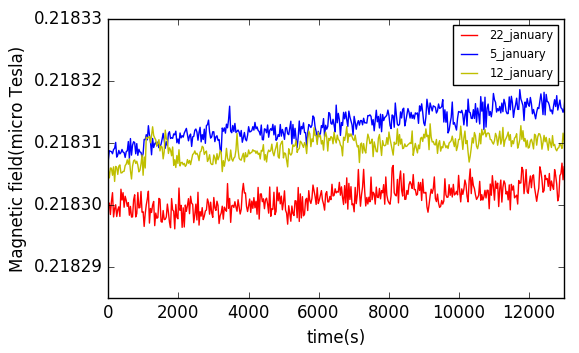
\includegraphics[width=0.85\linewidth]{figures/field_3_day}
\caption{Magnetic field recorded over 4 hours on three different
  days. The observed field drift is similar ($\sim 15$~pT) for each
  day.\label{fig:long-term-field}}
\end{figure}

Fig.~\ref{fig:long-term-field} shows the magnetic field recorded over
4 hours on three different days. Each data points in the graph
corresponds to a single FID measurement.  The observed field drift is
similar ($\sim 15$~pT) for each day.  The measurement was conducted at
0.2 $\mu$T magnetic field.

\begin{figure}%[h]
\centering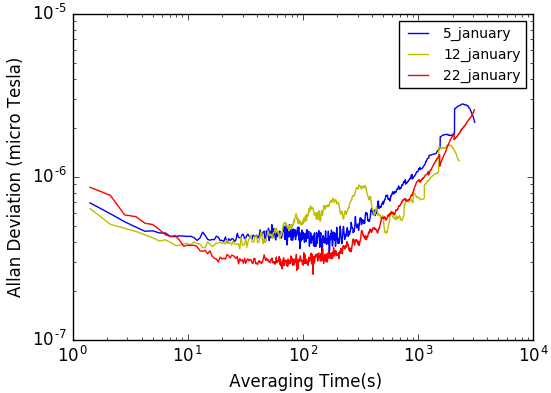
\includegraphics[width=0.8\linewidth]{figures/field_3_day_allan.png}
\caption{Allan deviation of recorded magnetic field vs.~averaging time
  for the time-series data presented in in
  Fig.~\ref{fig:long-term-field}.\label{fig:allan_deviation}}
\end{figure}

The Allan deviation was used to further quantify the long-term
stability~\cite{doe:website2} (see also Appendix~\ref{sec:appendix}).
Allan deviations characterize changes in the measured quantity when
the data are averaged on different timescales.  When the data behave
statistically on short timescales, the Allan deviation is equal to the
standard deviation.  If drifts occur, normally on longer timescales,
the Allan deviation grows linearly with a slope that $1/\sqrt{2}$
times the slope of the drift in time.

Fig.~\ref{fig:allan_deviation} shows the Allan deviations of the
measurements field presented in Fig.~\ref{fig:long-term-field}.  The
minimum in the Allan deviation occurs when statistical behavior is
overtaken by drift.  Fig.~\ref{fig:allan_deviation} shows that this
transition generally occurs after 10-60~s of averaging, corresponding
to a precision in magnetic field of 300-500~fT at the Allan minimum.

For an nEDM experiment, the goal precision is $\sim 20$~fT for the
average field over as measured over the 100~s neutron free-precession
measurement cycle.  This is not likely to be equivalent to the Allan
deviation minimum of our one magnetometer, because the long-term drift
is driven in part by the drift of the magnetic field within the
shield.  The goal of subsequent work was:
\begin{itemize}
\item to attempt to identify some of the sources of drift.  This
  included searching any sources that might be caused by the
  magnetometer itself, but also included the effects of
\item to improve the single FID performance so that fields could be
  measured faster.
\end{itemize}
In terms of the Allan deviation, it means trying to move the Allan
minimum lower and to the right.

\section{Optimization of cycle time\label{sec:optimization}} 

The goal of this optimization study was to reduce the cycle time
without sacrificing too much precision in the single-FID frequency
measurement.  If more measurements can be made more quickly, the
precision of the magnetometer over time would be improved.

\begin{figure}
\centering
\begin{subfigure}[b]{0.7\textwidth}
  \centering
  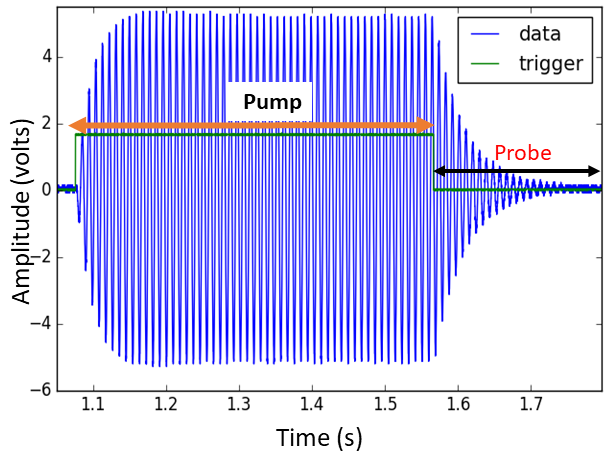
\includegraphics[width=\textwidth]{figures/FID_.png}
  \caption{}
  \label{fig:pump-long}
\end{subfigure}
\hfill
\begin{subfigure}[b]{0.7\textwidth}
  \centering
  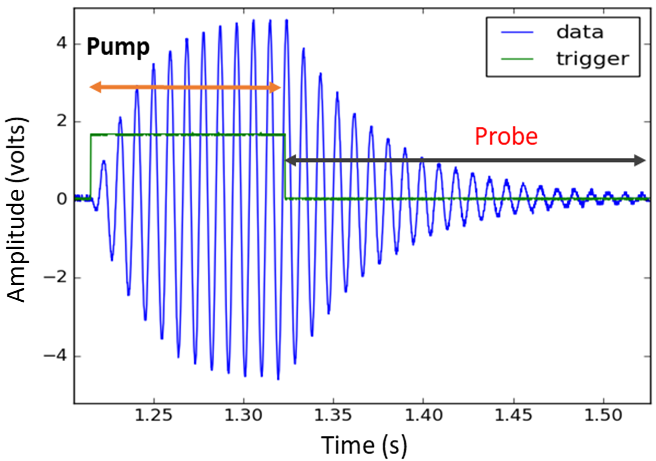
\includegraphics[width=\textwidth]{figures/Capture.png}
  \caption{}
  \label{fig:pump-short}
\end{subfigure}
\caption{(a) FID signal for pump time 0.49~s and probe time 0.4~s. (b)
  FID signal for pump time 0.1~s and probe time 0.2~s.  Both
  measurements were conducted at $0.2~\mu$T magnetic field.}
    \label{fig:pump-time}
\end{figure} 


During this study the magnetometer was operated in FID mode at
0.2~$\mu$T field.
%A complete cycle of FID measurement consist of a
%pump time followed by a probe time.  Pump time represents the time
%atoms take to generate a polarized ground state. In this study we were
%trying to study how long the optical pumping of Rb atom should have
%continued in order to generate an alignment and optical pumping for
%long time does make any difference in measuring magnetic field
%precisely or not.
An example of our initial settings is shown in
Fig.~\ref{fig:pump-long}.  The pump time is 0.49~s and the probe time
is 0.4~s.  The amplitude of the differential photodiode signal is seen
to saturate well within 0.1~s.  The coherence time, indicated by the
decay time of the oscillating signal, is about 0.06~s.
Fig.~\ref{fig:pump-short} shows a more optimized the FID signal for
0.1~s pump time and 0.2~s probe time.
\begin{figure}%[h]
  \centering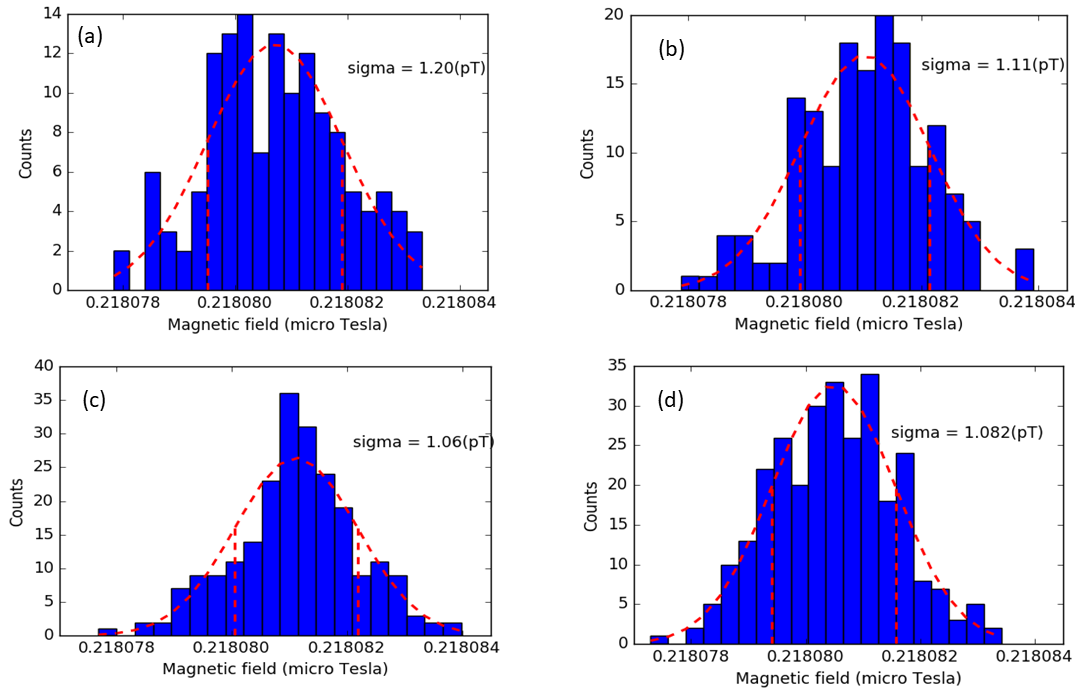
\includegraphics[width=\linewidth]{figures/pump_time_}
  \caption{Histograms of measured B-field for different pump times,
    for a measurement time of 100~s.  (a) is a pump time of 0.49~s (b)
    is a pump time of 0.39~s (c) is a pump time of 0.2~s (d) is a pump
    time of about 0.1~s.  The probe time in each case is about 0.25~s.
    The number of measurements taken in each case is estimated to be
    (a) 137 (b) 158 (c) 224 (d) 287.  The standard deviation of each
    set of measurements is indicated in the respective
    figure.}\label{fig:different-pump-time}
\end{figure}

In Fig.~\ref{fig:different-pump-time} a histogram of measured magnetic
fields by making subsequent measurements over 100~s is shown for
different pump times.  The longer pump time is 0.49~s
(\ref{fig:different-pump-time}(a)) and the shorter one is 0.1~s
(\ref{fig:different-pump-time}(d)).

From Fig.~\ref{fig:different-pump-time}, the pump time, when varied
over this limited range, does not strongly affect the precision of the
individual FID measurements.  However, it allows us to take
measurements faster because previously the duration for one FID
measurement was 1~s while after optimization it only take 0.35~s.

It is not surprising that the precision does not change much because
the amplitude of the differential photodiode signal during the pump
phase has saturated.

%In Fig.~\ref{fig:pump-long} the optical pumping is done for 0.49 s
%while signal amplitude reach its maximum over 0.1 s and after that
%signal amplitude remains unchanged till 0.49 s. In this case there is
%no point to pump more than 0.1 s. Same situation happens about probe
%time. If signal amplitude decays so quickly there is no point to set
%longer probe time. By optimizing pump and probe time we can speed up
%data acquisition system. After optimization for a single FID scan it
%only takes 0.35 s without losing any information. By using this faster
%data acquisition system it is possible to record multiple FID run with
%in a short period of time which is helpful to gather more information
%about magnetic field environment and helpful to achieve statistical
%precession.


\section{Magnet field compared with current in the $z$-coil}

\subsection{Current drift\label{sec:current-drift}}

\begin{figure}%[h]
\centering
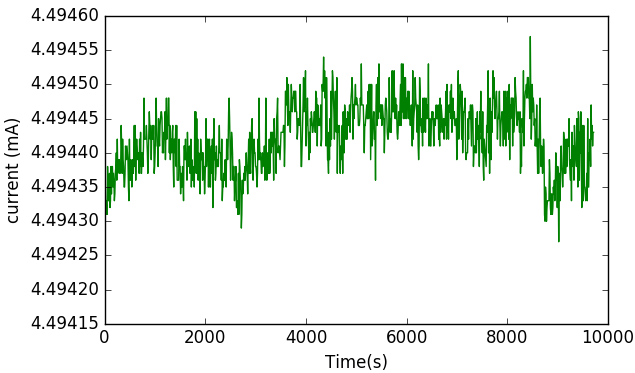
\includegraphics[width=0.7\linewidth]{figures/current}
\caption{Recorded coil current (by measuring voltage across a
  100~$\ohm$ resistor in series with the $z$-coil) as a function of
  time when the current source has been set to
  4.50000~mA.\label{fig:current}}
\end{figure}

The idea was to determine the impact of possible current drifts.  An
Agilent B2962A power supply was used to supply DC electrical current
to the $z$-coil.  Fig.~\ref{fig:current} shows the current supplied to
the $z$-coil over a measurement period of 10000~s.  The current in the
power supply was set to 4.50000~mA, which was operated in a
current-controlled mode.  The current has been measured by measuring
the voltage drop across a Vishay metal-foild 100~$\ohm$ resistor in
series with the $z$-coil using a Keithley 2002 8-digit multimeter.  A
photograph of this system is shown in
Fig.~\ref{fig:Current_study_setup}, although with an alternate
resistor which we tried.  The Vishay resistor is 1\% absolute
precision, but the values reported in Fig.~\ref{fig:current} have been
converted to currents using an exact value for the resistance of
100.000~$\ohm$.  The main feature of this resistor is that it
possesses a low temperature coefficient of 2~ppm/$\degree$C.
Measurements recorded by this system are expected to be reliable on
the $\sim\pm 2$~ppm level given the resistor and multimeter being used
and the typical temperature fluctuations in the room.


\begin{figure}%[h]
\centering
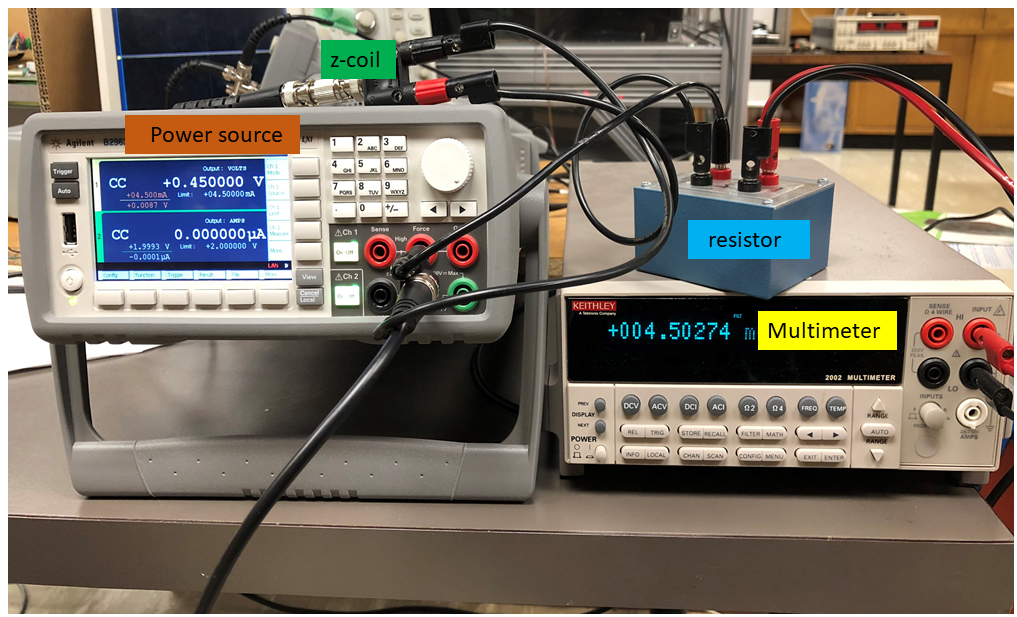
\includegraphics[width=\linewidth]{figures/current_study_setup.png}
\caption{Photograph of equipment arrangement used to control and
  measure the current in the $z$-coil.\label{fig:Current_study_setup}}
\end{figure}

The current of 4.5~mA achieves a magnetic field of 0.2~$\mu$T.  From
Fig.~\ref{fig:current}, the maximum current excursion during the
measurement period was 300~nA.  Likely these fluctuations are given by
the stability of the power supply. Converted to magnetic field, it
would represent a $\sim 10$~pT fluctuation in field.  Unfortunately,
during this measurement time, the magnetometer and degaussing system
could not be operated sufficiently well in concert with the current
measurement system to determine whether or not the current
fluctuations were correlated to field changes.  Principally this was a
problem of the data acquisition system.  Clearly, field changes as
large as 10~pT should be observable, given the statistical precision
of the magnetometer.  Future work would be on improving the data
acquisition system.

%\begin{figure}
%  \centering
%  \begin{subfigure}[b]{0.67\textwidth}
%    \centering
%    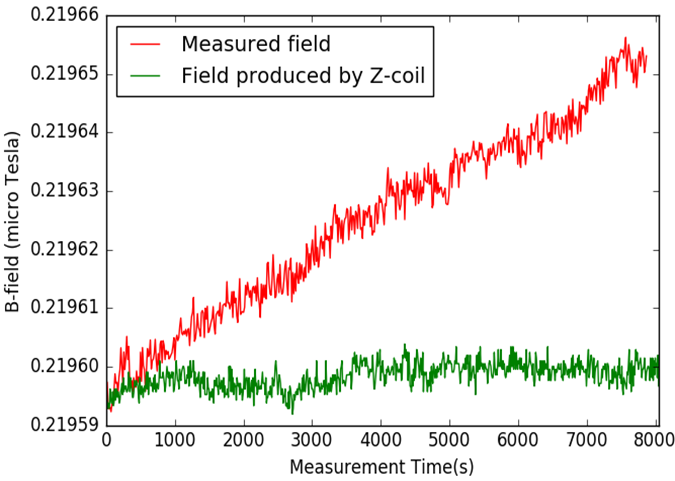
\includegraphics[width=\textwidth]{figures/field_coil_current.png}
%    \caption{}
%    \label{fig:field_measure_and_produced}
%  \end{subfigure}
%  \begin{subfigure}[b]{0.65\textwidth}
%    \centering
%    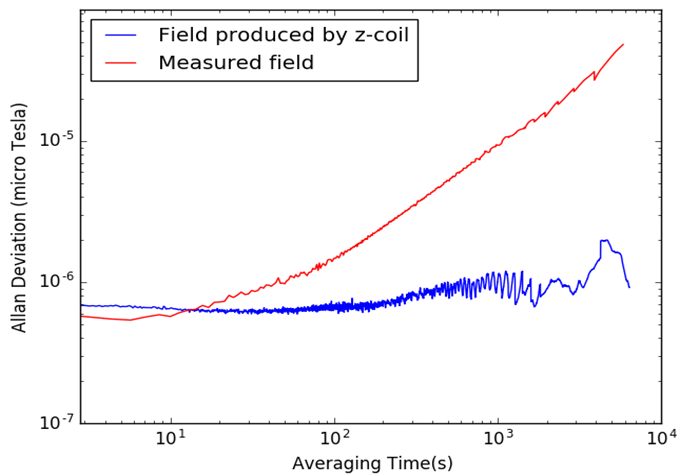
\includegraphics[width=\textwidth]{figures/field_current_allan_plot.png}
%    \caption{}
%    \label{fig:allan_plot}
%  \end{subfigure}
%  \caption{(a) (Blue) Measured current in the $z$-coil converted to
%    field, using the normalization constant measured at 0~s.  (Red)
%    Measured magnetometer frequency converted to field using the
%    gyromagnetic ratio of $^{85}$Rb.  (b) Allan deviation of of the
%    time series in (a).}
%  \label{fig:current_vs_field_allan_deviation}
%\end{figure} 

%Fig.~\ref{fig:field_measure_and_produced} displays the magnetic field
%measured by the magnetometer over the same period.  The magnetometer
%was operated in FID mode as usual and the magnetometer settings were
%similar to those used in Section~\ref{sec:long-term}.
%%{\bf list all settings, lock-in time constant, laser power, lock-in
%%  frequency, magnetometer measured frequency, etc.}
%%produced by z-coil(green line) and measured field (red line) by
%%running the magnetometer in FID mode over 8000 s.
%The field produced by the $z$-coil is calculated by converting
%measured current to field with the coil constant measured at $t=0$~s.
%At $t=0$ both fields are therefore forced to coincide and over time a
%linear drift can be seen in the field measured by the magnetometer,
%while the current in the $z$-coil would indicate that the field should
%not be changing.  Interestingly, aside from the overall drift, there
%might be some correlation of excursions in the current with excursions
%in the magnetometer reading.  The interpretation is somewhat obscured
%by the drift.  Also the exact time synchronization of the current data
%and the field measurement data was not tested precisely, and may have
%some relative time drift.

%For a better understanding of the stability of the power supply the
%Allan deviation of the field produced by the $z$-coil (deduced by its
%current) and the field measured by the magnetometer are shown in
%Fig.~\ref{fig:allan_plot}.  It can be seen from the figure that for
%long times, the current stability is better than typical measured
%field changes.  At short times, the current stability is considerably
%worse than the field stability.  This might be due to additional noise
%in the current measurement system, or a different bandwidth being used
%for the current measurement system.


%{
%\bf How is the coil current measured? 
%%Coil current was measured by using a Keithley 2002 multimeter.
%Why was the coil current
%  measured for longer than the field?  Was the coil current averaged
%  over the same time as each frequency measurement? 
%  % yes averaging time is same for current and frequency.
%  Why is the
%  current noisier than the magnetometer for short averaging times in
%  the Allan deviation? 
%  
%  How were the current and field data acquired?
%  How were the data synchronized to one another in time?  How is the
%  measurement time defined for the coil current?  Is it at the start
%  of the FID measurement or the end of the FID measurement, or
%  somewhere in the middle, or asynchronously?  For the FID
%  measurements, which time is graphed?  The start, end, or half-way
%  time, or at the 1/e time of the FID?  Please show the measured coil
%  current in the next section as well for
%  Fig.~\ref{fig:field-change}.}



\subsection{Change in magnetic field driven by larger changes in coil current}

A study was conducted to determine the field change by changing the
coil current by a known amount. The main objective of this study is to
confirm the Rb magnetometer performance on magnetic field measurement.
For this measurement coil current was changed periodically by $\pm
0.001$~mA steps.  Based on the coil constant, field changes of 48~pT
were expected to be observed in the magnetometer, corresponding to
frequency shifts of 0.5~Hz.

The laser frequency was tuned for maximum FID amplitude, then locked
using the DAVLL system.  All other magnetometer settings were similar
to the previous studies in Section~\ref{sec:current-drift}.  During
this study the magnetometer has been operated in FID mode.  The
lock-in frequency was 1950 Hz and time constant was 300~$\mu$s.  The
AOM frequency was tuned initially to maximal optical rotation and
found to be 2049~Hz.  The probe beam power was 20~$\mu$W and pump
power $\sim 40~\mu$W.  The pump and probe times were both 0.5~s.  Only
X data was fitted to determine the magnetometer frequency.

\begin{figure}%[h]
\centering
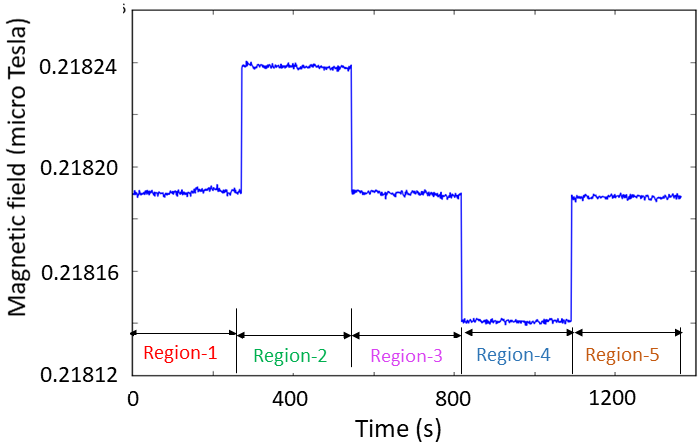
\includegraphics[width=0.7\linewidth]{figures/field_change-with-current}  
\caption{Change in magnetic field measured by the magnetometer by step
  changes in the $z$-coil current.  In Regions 1, 3, and 5, the
  current was set to 4.50000~mA on the power supply.  In Region 2, the
  current was changed to 4.50100~mA.  In Region 4, the current was
  4.44900~mA.\label{fig:field-change}}
\end{figure} 
 
Fig.~\ref{fig:field-change} presents the magnetic field change over
time for different coil current. For better understanding
Fig.~\ref{fig:field-change} has been divide into five different
regions where a number of different coil currents were set near
4.50000~mA in steps of 0.00100~mA.  It is clear from the figure that
the field has been changed by $\sim 50$~pT on each transition.  This
measurement proves rather conclusively that changes in the magnetic
field with large current changes are indeed reproduced correctly.  It
should be noted that up to 30~s of data of been omitted near each
transition.


\section{Study the effect of room temperature in magnetic field\label{sec:temperature}} 

The goal of this study was to search for any correlation between the
magnetic field measured by the magnetometer and ambient temperature
flucturations near the magnetometer.

\begin{figure}%[h]
\centering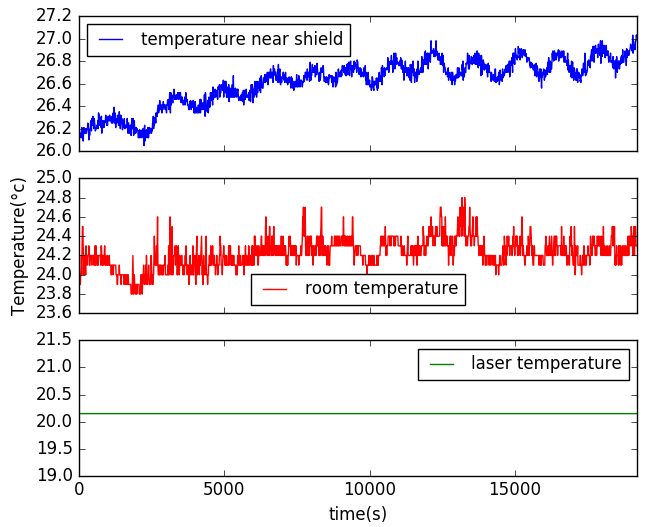
\includegraphics[width=0.8\linewidth]{figures/temp_.png}
\caption{Temperature measurements as a function of time.  The upper
  graph (blue) shows the temperature measured on the outermost
  magnetic shield.  The lower graph (red) shows the temperature in the
  room outside the laser hut, near the power supply and function
  generator system.\label{fig:temperature-measurement}}
\end{figure}

Fig.~\ref{fig:temperature-measurement} displays the measured
temperature at various locations vs.~time.  It can be seen that room
temperature fluctuations are 1\degree{C} while temperature measured on
the outside of the magnetic shielding is about 0.8\degree{C}.  The
optics table is covered by a clean enclosure, which makes the
temperature measured on the top of the magnetic shield slightly warmer
than the rest of the room.  The temperature on top of the shield is
measured by a T-type thermocouple that was held to the shield using
tape and thermally connected by thermal grease.  We often use T-type
thermocouples because they are non-magnetic, as opposed to K-type
which are magnetic.

For room temperature measurement a precision thermometer was connected
to a Agilent 34410A 6$\frac{1}{2}$ Digit Multimeter.  A Python script
configured the multimeter for a 2-wire RTD measurement, triggered the
meter, and transferred the reading to the computer.  The T-type
thermocouple on the shield was connected to an Arduino Uno.  For
configuring this device and then transferring the reading to the
computer a different part of the same Python script was used.  After
an acquisition of the two temperatures, the script paused for 10~s, so
that measurements came approximately every 12.3~s.

%The laser diode temperature was read by the output of the temperature
%control unit for the Toptica laser using another oscilloscope and
%converted to temperature using a known coefficient.  Since it did not
%vary with time it was not considered further.

\begin{figure}%[h]
\centering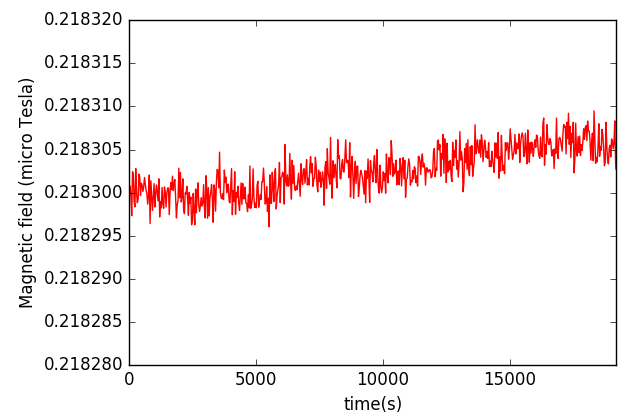
\includegraphics[width=0.8\linewidth]{figures/field_.png}
\caption{Field measurement\label{fig:field}}
\end{figure}

Fig.~\ref{fig:field} shows the magnetic field measured by the
magnetometer in FID mode vs.~time in similar times as the temperature
measurement was made.  The magnetometer settings were the same as in
the previous section, with the caveat that the frequency of the AOM
was adjusted for best FID amplitude (2036~Hz) and lock-in adjusted to
keep the FID demodulated frequency near 90~Hz (1929.5~Hz).

The FID measurements were taken using an oscilloscope.  The
oscilloscope would be read occasionally.  No data is shown twice in
Fig.~\ref{fig:field}, but time jumps in the data did occur at random
intervals.  Thus any correlation with temperature is qualitative.  The
meausrements were taken over approximately the same time as the
temperature measurements.

The asynchronous data acquisition systems mean that time was defined
with factor of 2 level accuracy.  Nonetheless, a the correlation of
the field measurement is ruled out at approximately the
5~pT/\degree{C} level.


%Temperature change and field change, the measured field
%vs.~temperature has shown in Fig.~\ref{fig:field_vs_temp}. {\bf What
%  was the data acquisition system for each device?  How were the data
%  synchronized?%   }  It is clear from the graph
%that there is no obvious of field drift dependency on temperature.

%\begin{figure}%[h]
%\centering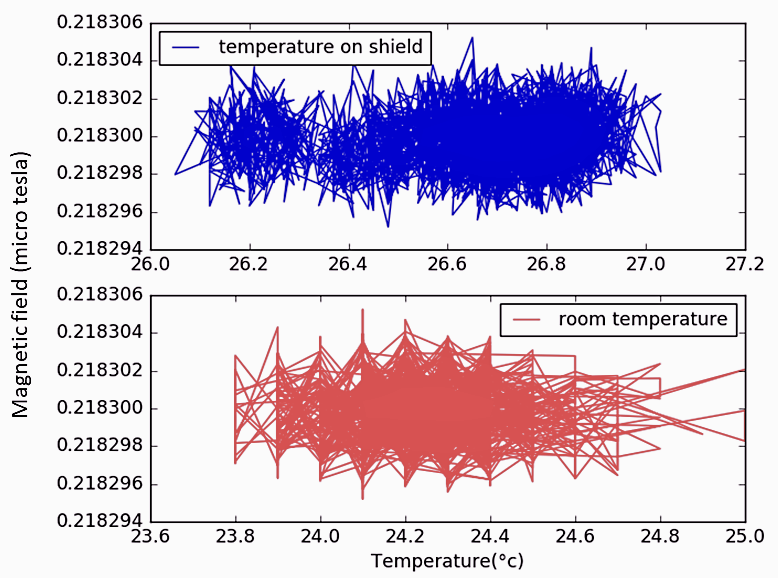
\includegraphics[width=0.6\linewidth]{figures/field_vs_temp.png}
%\caption{Field vs. temperature\label{fig:field_vs_temp}}
%\end{figure}
 
   
\section{Degaussing studies\label{sec:degaussing}}

\subsection{Initial tests using the magnetometer near zero field\label{sec:degauss-near-zerofield}}

%different degaussing schemes(changing sample rate)
   
  
%Degaussing process is done in order to avoid the environmental
%perturbation and reduce any remnant field inside the four layer $\mu$
%metal magnetic shield \cite{doi:10.1063/1.2713433}. The setting for
%degaussing has shown in Table \ref{table:degaussing-setting}.  A
%detailed analysis of NMOR signal by changing the degaussing parameter
%could give us some information about the goodness of degaussing
%procedure. Toward this end, a study has been carried out to determine
%the dependency of the resonance width on the sample rate (see
%discussion on section \ref{sec:Degaussing}).

We used the procedure described in Section~\ref{sec:near zero field}.
To remind the reader, the procedure is:
\begin{itemize}
\item Initiate the degaussing sequence in one channel of the function
  generator.
\item Once complete, ramp the rheostat to zero and open the switch.
\item Pressing a button on the computer initiates the ramp of the
  $z$-coil on the second channel of the function generator, which
  calibrates the optical rotation to field.
\item Both the current in the $z$-coil and the differential photodiode
  signal are monitored at all times using an oscillscope.
\end{itemize}

%In this study, data was acquired by sweeping the magnetic field near zero field. Before each measurement degaussing the innermost layer of shield has done. During this measurement only one degaussing parameter, sample rate, was varied in order to study the effect of degaussing parameter on magnetic field measurement.  

\begin{figure}%[h]
  \centering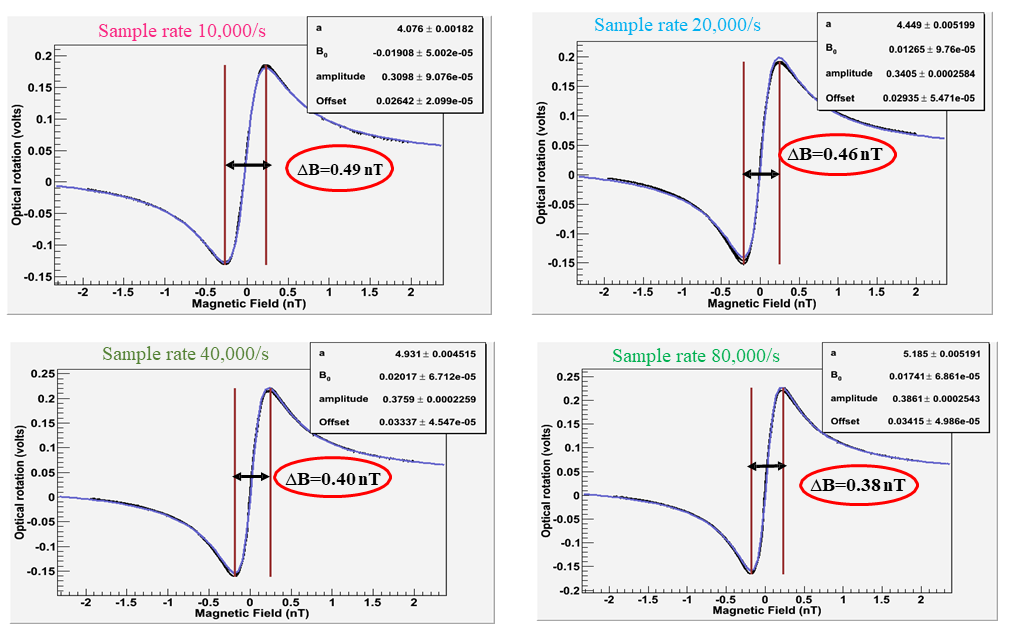
\includegraphics[width=\linewidth]{figures/sample_rate}
  \caption{ Optical rotation vs. measured B-field for different sample
    rate.  The data were taken in order from smaller sample rate to
    higher sample rate.  The numbers written in the red circles
    indicate the distance in magnetic field from the optical rotation
    minimum to the optical rotation maximum $\Delta B$, as deduced
    from the fit parameter $a$.  The fit parameter $B_0$ indicates the
    remnant field sensed by the horizontal offset of the dispersive
    shape, reported in nT.\label{fig:different-sample-rate}}
\end{figure}

Optical rotation as a function of magnetic field for different sample
rate is shown in Fig.~\ref{fig:different-sample-rate}.  Recall that
the sample rate determines the rapidity with which the $5\times 10^5$
individual samples of the linear degaussing envelope function are
stepped through.  A sample rate of 10,000/s therefore represents a
degaussing time of 50~s.  Since the carrier wave in all cases is
10~Hz, it means that 500~cycles were used.  The sample rate of
80,000/s represents a degaussing time of 6.25~s and 62.5 cycles.

It should also be noted that the data were acquired in order of
increasing sample rate, and that many additional degaussing sequences
were conducted which are not shown in
Fig.~\ref{fig:different-sample-rate}.

We had expected that larger sample rate would manifest itself as a
worse degaussing resulting possibly in worse magnetometer performance.
Paradoxically, the resonance width $\Delta B$, the difference between
two peak of the dispersive curve, reduced very slightly as the sample
rate was increased.  It can be seen from
Fig.~\ref{fig:different-sample-rate} that, the resonance width is
about 0.49~nT for sample rate 10,000/s and the resonance width is
0.38~nT for sample rate 80,000/s.  This is likely an indication of a
small reduction in the transverse fields or generally an improvement
the homogeneity of the field.  This is consistent with the observation
that the amplitude grows slightly, which is another indication of the
improved field quality, all other magnetometer settings being equal.

The remnant field $B_0$ is an indication of the average longitudinal
field (along the laser beam axis) and is within 20~pT of zero.  It
increased with the sample rate from a starting negative value to a
positive value.

The conclusion of this study was that additional degaussing, as long
as it has a reasonable number of cycles, tends not to affect the field
or it might improve slightly the homogeneity of the field.  Generally
the field is reduced below 20~pT.

%\begin{figure}%[h]
%\centering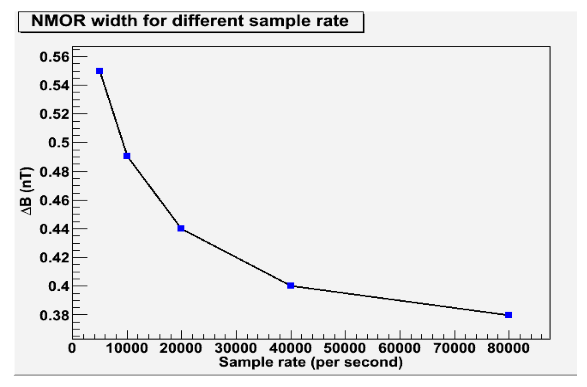
\includegraphics[width=0.6\linewidth]{figures/field_vs_sample_rate}
%\caption{Resonance width vs.~sample rate. Resonance width decreases
%  with increasing sample rate.  When the sample rate is 5000~samples/s
%  the observed resonance width is 0.55~nT. On the other hand the
%  resonance width is 0.38~nT for sample rate 80000
%  sample/s. \label{fig:resonance width vs. sample rate} }
%\end{figure}

%Fig~\ref{fig:resonance width vs. sample rate} shows the resonance
%width as a function of sample rate. Resonance width decreases with
%increasing sample rate.  It is obvious from the graph that the
%resonance width becomes narrower for larger sample rate.

\subsection{Measurements at 0.2~$\mu$T and initial studies of the effect of degaussing on field stability\label{sec:three-degauss}}


The previous results implied that additional (even poor) degaussing
had little impact if the previous degaussing was done adequately.  To
address this, we began to do studies where the internal $z$-coil field
was purposely ramped to a large value, then reset to a low value for
measurements at non-zero field.  The idea here was to use the $z$-coil
itself to magnetize the shields, and to measure drifts at non-zero
field, which is the chief interest for nEDM experiments.

%A study has conducted by making the magnetic field environment bad
%inside the shielding intentionally by ramping the field from a lower
%value to higher value and observe any change in field drift. This
%study has done in 3-steps:
%  \begin{itemize}
%      \item take field measurement for about 2000 s without performing any degaussing.
%      \item Intentionally make the field environment bad and take field measurement for another 2000 s. No degaussing has done in this step also.
%      \item perform degaussing of the innermost shield and again measured magnetic field for 2000 s.
%  \end{itemize}

\begin{figure}
  \centering
  \begin{subfigure}[b]{0.48\textwidth}
    \centering
    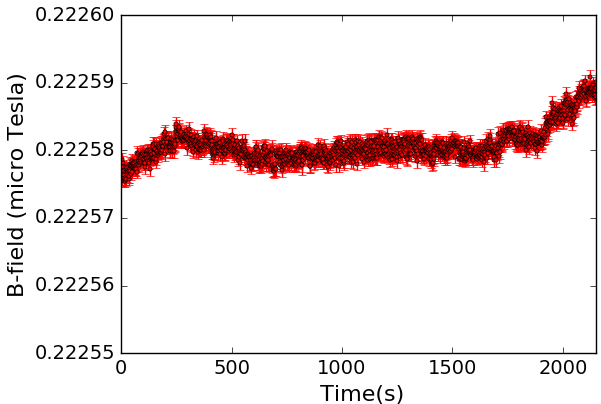
\includegraphics[width=\textwidth]{figures/ramp_1}
    \caption{}
    \label{fig:ramp-up}
  \end{subfigure}
  \hfill
  \begin{subfigure}[b]{0.48\textwidth}
    \centering
    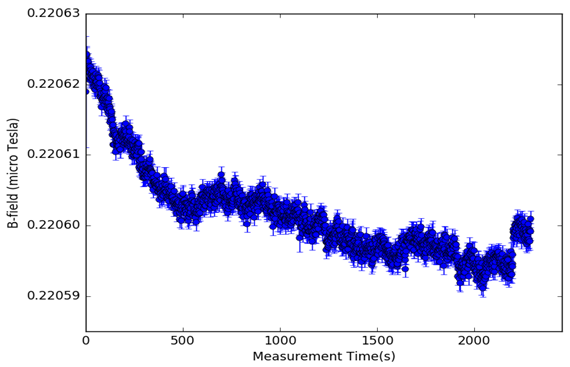
\includegraphics[width=\textwidth]{figures/ramp_2}
    \caption{}
    \label{fig:ramp-down}
  \end{subfigure}
  \begin{subfigure}[b]{0.48\textwidth}
    \centering
    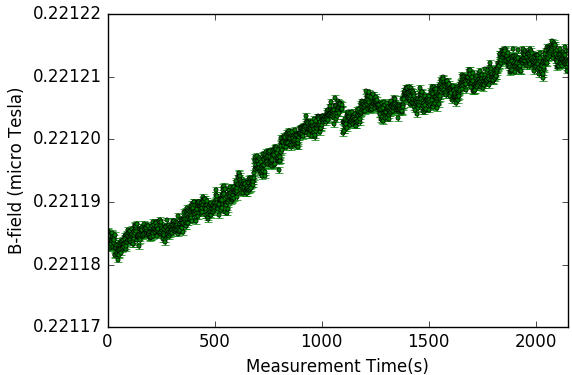
\includegraphics[width=\textwidth]{figures/ramp3}
    \caption{}
    \label{fig:degauss}
  \end{subfigure}
  \caption{Measurements conducted in time order from (a) to (b) to (c)
    under different degaussing conditions at $B_z=0.2~\mu$T magnetic
    field: (a) no degaussing, (b) ramp $B_z$ from 0.2~$\mu$T to
    10~$\mu$T then again set it to 0.2~$\mu$T and collect FID signal
    before degaussing, and (c) after degaussing.}
  \label{fig:ramp-updown}
\end{figure}

Fig.~\ref{fig:ramp-updown} shows an example of such a study.  In all
three cases shown in Fig.~\ref{fig:ramp-updown}, the magnetometer
settings are similar in each case.  The AOM frequency was adjusted
slightly to optimize the FID amplitude for each measurement, but the
lock-in frequency and most other settings were left the same.
%Since the field changed in each measurement, the magnetometer was
%retuned each time, principally the pump frequency and the lock-in
%amplifier internal reference frequency.  {\bf What are the
%  magnetometer settings?}
 % AOM frequency 2064 Hz and lock-in frequency 1950.2 Hz (fig:5.12(a))
 % AOM frequency 2059 Hz and lock-in frequency 1950.2 Hz (fig:5.12(b))
 % AOM frequency 2078 Hz and lock-in frequency 1950.2 Hz (fig:5.12(c))
  
In the 1st part of this study the magnetometer was operated in FID
mode at 0.2~$\mu$T field, at a point in time when the magnetometer had
been operated in a quiet shielded environment for at least a month
below 1~$\mu$T, over the course of which the shield had been degaussed
a number of times.
  
The recorded magnetic field measurement over a 2200~s period in this
condition is shown in Fig.~\ref{fig:ramp-up}.  It can be seen from
Fig.~\ref{fig:ramp-up} that the magnetic field increased linearly for
first 300~s then showed a decrease in field. The field was pretty
stable between 600~s and 1800~s and after that the field showed an
increase. The overall field change is about 15 pT during the
measurement.  In Fig.~\ref{fig:ramp-down}, data was acquired by
ramping $B_z$ from 0.2~$\mu$T to 10~$\mu$T then down again to
0.2~$\mu$T and collect FID signal.  Since the $z$-coil is coupled to
the inner shield system, this should magnetize the shields.  By doing
this field ramping we intentionally perturb the magnetic field
environment inside the shield.  After this field ramping the long term
field measurement has been conducted for another 2200 s. In this case,
the field showed a downward drift of about 35~pT.  Thus field ramping
did seem to change the magnetic environment inside the magnetic
shielding.

Finally, for Fig.~\ref{fig:degauss}, the innermost
magnetic shield was degaussed  with degaussing parameters stated in Table \ref{table:degaussing-setting}
Before starting field measurement via FID mode degaussing was done multiple times (4-5 times) repeatedly but during the measurement no degaussing was done. 
  
While this changed the direction of the drift, it did not change the
magnitude of the drift which was again 35~pT over 2200~s.
%  {\bf Is it true that no amount of degaussing of the innermost
%  shield changed this significantly? It could.  I have tried to
%  degaussing multiple times but I never find the evidence of solving
%  the field drift problem significantly by degaussing the innermost
%  layer. Usally I saw that after degaussing the error bar goes down}

% I cannot tell what was done or observed so I recommend not to make
% any particularly bold statement like the one I was suggesting.

During this time we began to develop a hypothesis about magnetic
couplings inside the magnetic shielding.  We realized that the
$z$-coil, which had been designed to be coupled to the innermost
shield, was now more strongly coupled to the second innermost shield.
This is because most of the flux in the solenoidal winding exits the
end of the innermost shield, whose endcaps have been removed in order
to accommodate its degaussing coil.


\subsection{Effect of degaussing the three outermost shields\label{sec:outermosts-shield-degauss}}
 
If the system had been kept at low field for several days, the usual
field drift was about 15 pT over 3000~s (as discussed in
Sections~\ref{sec:three-degauss} and~\ref{sec:long-term}).  After
doing a transverse field study (applying current to $x$- and $y$-coils
along with $z$-coil, like that reported in
Sections~\ref{sec:ch4_tilted_field} and~\ref{sec:tilted-results}) the
magnetic field environment became even more unstable.

\begin{figure}
  \centering
  \begin{subfigure}[b]{0.48\textwidth}
    \centering
    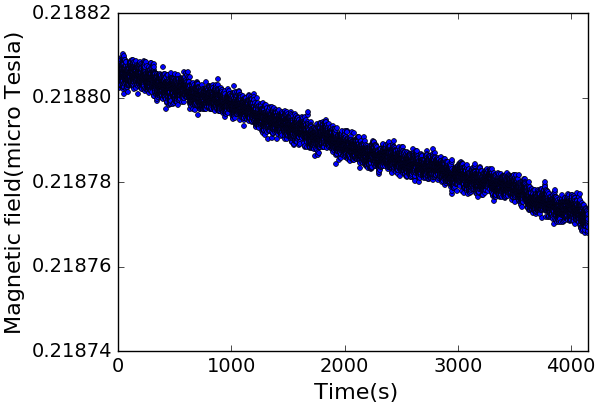
\includegraphics[width=\textwidth]{figures/before_degaussing}
    \caption{}
    \label{fig:with DG_innermost}
  \end{subfigure}
  \hfill
  \begin{subfigure}[b]{0.48\textwidth}
    \centering
    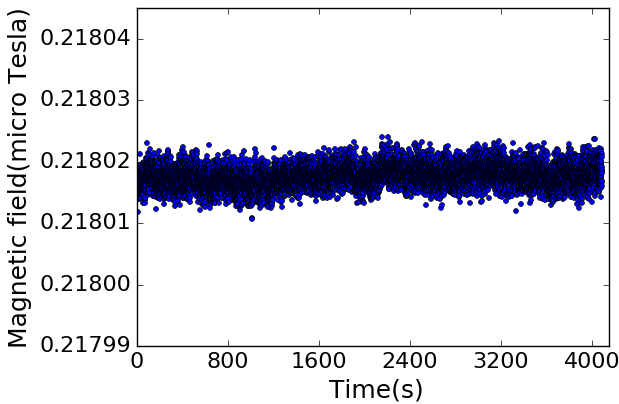
\includegraphics[width=\textwidth]{figures/after_degaussing.png}
    \caption{}
    \label{fig:with DG}
  \end{subfigure}
  \caption{Magnetic field vs.~time (a) after degaussing the innermost
    shield, and (b) after additionally degaussing the remaining layers
    of magnetic shielding with a single loop of wire wound through all
    three layers. During this study the signal amplitude was
    relatively low ($\sim 3$~V) likely due to poor laser alignment
    through the AOM or other settings. As a result the fluctuations in
    magnetic field were larger than the usual 1-2~pT.\label{fig:effect
      of DG}}
\end{figure}

Fig.~\ref{fig:with DG} shows about 50~pT drift in magnetic field in
4000~s. Although before start taking field measurement degaussing
innermost layer of mu-metal is done multiple times in order to cancel
background field inside the shield but still the field drift problem
can be seen. Then degaussing the other three shielding layers is done
with a single loop of wire wound through all three.  The maximum
current achieved in this coil was equivalent to the maximum current in
the innermost shield deguassing sequence.  However since a single loop
is wound through all three outermost shields, it is unlikely that any
of the three shielding layers are ever saturated.  Nonetheless, this
seemed to reduce the field drift after degaussing the outer three
shielding layers, as shown in Fig.~\ref{fig:with DG}). During those
measurements the lock-in reference frequency was set to 1938.5~Hz and
lock-in time constant is 300~$\mu$s.

%Since the endcap of the innermost shield layer was removed, the
%$z$-coil may magnetize the second-to-innermost shield.  We expect this

The conclusion is that degaussing the outer three shields is equally
as important as the degaussing of the innermost shield.  This is not
surprising since the endcaps of the innermost shield were removed.

A side note is essentially that the design of magnetic components
placed inside the magnetic shields needs to be carefully considered.
It is clear that the degaussing system was designed after the magnetic
shields and the inner coil systems had been designed.  In itself this
is an error in the design process of the entire system which arose due
to a lack of understanding of the importance of degaussing.


\section{Laser tuning\label{sec:tuning}} 

In the course of tuning the laser for maximum FID amplitude, some
studies were conducted where the laser was purposely mistuned in order
to check the effect on the measured FID fit parameters.  In general,
for the particular magnetometer settings otherwise in use, it was
found that detuning from the maximum amplitude tended to increase the
coherence time (1/e decay time of the oscillating FID signal),
although on occasion shorter coherence times could be observed.  By
taking measurements in rapid succession, it was also found that the
FID frequency did not change considerably at the 0.01~Hz (sub-pT)
level.

We started doing studies like this because there was some (mistaken)
belief that the laser tune significantly altered the FID measured
frequency.  This was based on data like that shown in
Fig.~\ref{fig:digilock-drift}.

\begin{figure}%[h]
  \centering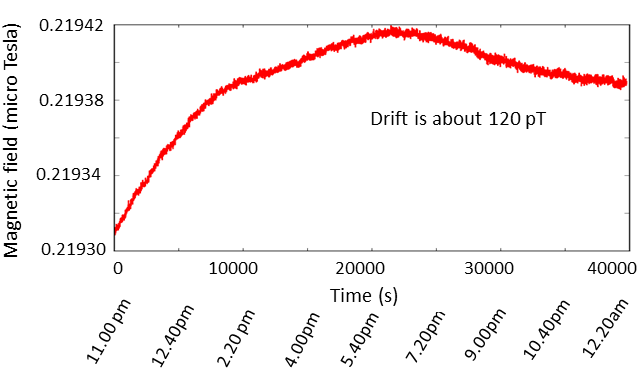
\includegraphics[width=0.8\linewidth]{figures/field-drift}
  \caption{Magnetic field recorded over 12~hours.  In this
    measurement the observed field drift is
    about~120~pT.\label{fig:digilock-drift}}
\end{figure}

Fig.~\ref{fig:digilock-drift} indicates a 120~pT drift in magnetic
field over 12~hours.  The laser frequency is believed to drift because
the amplitude of the FID decreased by a factor of 2.5 over the course
of the measurement, while the resonant frequency only changed by
1.5~Hz.  The fact that the amplitude has decreased is indicated by the
relevant fit parameter which is not shown, but can be seen from the
additional statistical noise on the field measurements at long times
compared to short times.  The question was if this possible drift in
tune was causing any frequency drift or not.

We suspected the tune might be drifting because we use a polarizing
beamsplitter cube in our DAVLL system which may possess poor stability
over long time periods~\cite{bib:Philip2008}.

In order to test the hypothesis that the frequency of the laser might
be drifting, I did a study where I manually adjusted the frequency of
laser light to maximize optical rotation.  The DAVLL and Digilock
system were not used to lock the laser during this study.  Rather,
periodically, the data acquisition was paused, and the laser frequency
was adjusted manually to maintain the same (largest) differential
photodiode amplitude. The data acquisition was then restarted.

\begin{figure}
  \centering
  \begin{subfigure}[b]{0.5\textwidth}
    \centering
    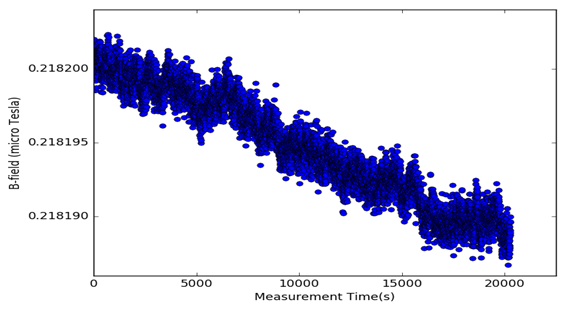
\includegraphics[width=\textwidth]{figures/manual_tuning}
    \caption{}
    \label{fig:field-manual-tuning}
  \end{subfigure}
  \hfill
  \begin{subfigure}[b]{0.49\textwidth}
    \centering
    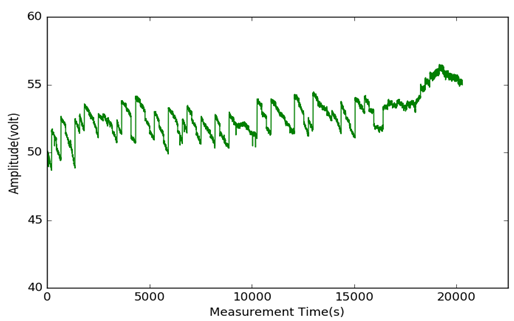
\includegraphics[width=\textwidth]{figures/amplitude_manual_tuning}
    \caption{}
    \label{fig:amplitude-manual-tuning}
  \end{subfigure}
  \caption{(a) magnetic field vs. time. (b)  Amplitude of recorded
    FID NMOR signal over 20000~s. During this study laser tuning is
    maintained manually, as can be seen from the jumps in the
    amplitude which occur upon retuning.}
  \label{fig:manual-tuning}
\end{figure}
   
The results of the measurement are shown in
Fig.~\ref{fig:manual-tuning}.  Fig.~\ref{fig:amplitude-manual-tuning}
shows the fitted initial amplitude (after the pump beam has been
switched off) as determined by the fit to the decaying oscillating
function.  The spikes in Fig.~\ref{fig:amplitude-manual-tuning}
indicate times when the retuning of the laser was conducted, as
described above.  A time jump (not shown) of a random by relatively
short interval also occurs for each retuning, which is not shown.

Fig.~\ref{fig:field-manual-tuning} shows the result of the frequency
measurement, when translated into magnetic field.  It can be seen that
as the amplitude of the fit decreases (presumably due to a drift in
the laser frequency), the statistical fluctuations in the field
measurement increase.  This would be expected because a small fit
amplitude will make the frequency statistically more difficult to
measure.

Clearly the field measurement in Fig.~\ref{fig:field-manual-tuning}
does not drift in the same way as the FID amplitude in
Fig.~\ref{fig:amplitude-manual-tuning}.  Thus we conclude that the
field measurement in FID mode is relatively insensitive to the
frequency tuning of the laser, except that if the tune drifts, the
frequency measurement becomes statistically less precise.

%we can say that during this measurement the amplitude
%of FID NMOR was pretty stable except small fluctuations over 20000 s
%. The observed small fluctuation is due to the manual adjustment while
%keeping the laser frequency tuned to atomic transition over long
%period of time. Obtaining stable signal amplitude is a indication that
%laser is not drifting to much. Although laser frequency was not
%drifting a lot during the measurement, still there is a drift in
%magnetic field (Fig.~\ref{fig:manual-tuning}). The overall drift is
%about 20~pT over 20000~s. So it can be conclude that the drift in
%laser frequency is not the main reason behind this induced field
%drift.


\section{Improving the precision of individual FIDs, and problems encountered in doing so\label{sec:reference-frequency}}

\subsection{Optimization of pump and probe beam power} 
A study has been performed to determine how optimization of the pump
and probe beam power effect on precise field measurement.  During this
study, the magnetometer has operated in FID mode.
\begin{figure}
  \centering
  \begin{subfigure}[b]{0.7\textwidth}
    \centering
    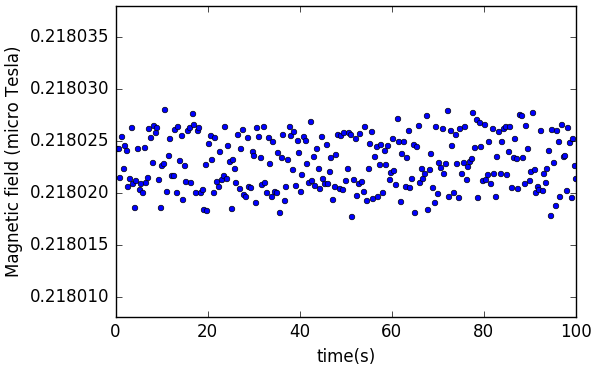
\includegraphics[width=\textwidth]{figures/beam_power_less}
    \caption{}
    \label{fig:power less}
  \end{subfigure}
  \begin{subfigure}[b]{0.7\textwidth}
    \centering
    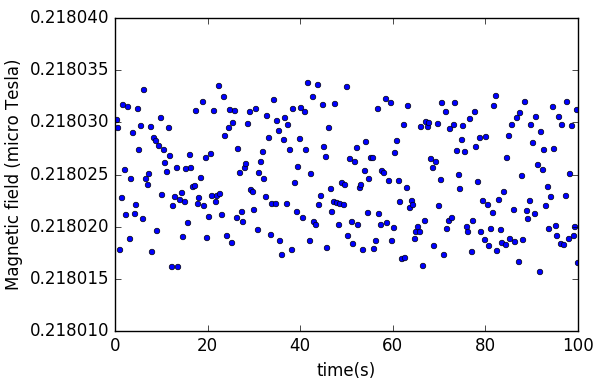
\includegraphics[width=\textwidth]{figures/beam_power_double}
    \caption{}
    \label{fig:power double}
  \end{subfigure}
  \caption{ Magnetic field as a function of time for different power
    of probe beam: (a) 15~$\mu$W, the standard deviation of the data
    is 3.01~pT (b) 30~$\mu$W, the standard deviation is
    7.2~pT.\label{fig:different probe power}}
\end{figure}
%data colllected 13th August 2018
 
In Fig.~\ref{fig:different probe power} the measured magnetic field
has been displayed for two different probe beam
power. Fig.~\ref{fig:power less} presents the measured field over
100~s with 15~$\mu$W probe power while Fig.~\ref{fig:power double}
display the measured field over 100~s for probe power 30~$\mu$W. In
both cases, the pump beam power the same ($\sim 40~\mu$W). Each blue
points in this graph represent a single FID scan. As can be seen from
Fig.~\ref{fig:different probe power} the magnetic field were more
scattered for high probe beam power.  The standard deviation of the
data was 7.2~pT for probe beam power 30~$\mu$W while for low beam
power of 15~$\mu$W the standard deviation was 3.01~pT.

\begin{table}%[h]
\centering
\begin{tabular}{|c|c|c|}\hline
\textbf{Probe power ($\mu$W)}    & \textbf{Coherence time (ms)}  & \textbf{Amplitude (V)}\\\hline
2 & 84 & 2.13   \\
5    & 82 & 2.11  \\
10   &  68 & 4.06 \\
15  &   59 & 5.8  \\
35  &   32 & 10  \\\hline
\end{tabular}
\caption{Single FID fit parameters as a function of probe beam
  power.\label{tab:coh}}
\end{table}

The apparently worse statistical precision for higher probe beam power
can be traced in part to its effect on the individual FID signals of
each measurement.  Table~\ref{tab:coh} displays the coherence time of
the FIDs for different probe power while the pump beam power was held
constand (120~$\mu$W).  For these settings, the coherence time is seen
to increase for descreasing probe power, which acts to improve the
statistical precision.  However, it is counteracted by a corresponding
decrease in the FID amplitude which acts to worsen the statistical
precision.  The trade off of these two effects must be considered when
selecting the probe power for a given pump power.  In general it is
expected that a probe power in the $\mu$W range would be optimal.
 
The effect of pump beam power was also studied with the probe beam
power ($\sim 15~\mu$W) held constant.  The pump beam power was changed
by changing the duty cycle of the square wave modulation used for the
AOM.  When duty cycle is set to 5\% the pump beam power is roughly
40~$\mu$W and for 16\% duty cycle power is roughly 130~$\mu$W. During
this measurement the lock-in reference frequency was set to 1943.9 Hz
while the AOM frequency was 2036~Hz.

\begin{figure}
  \centering
  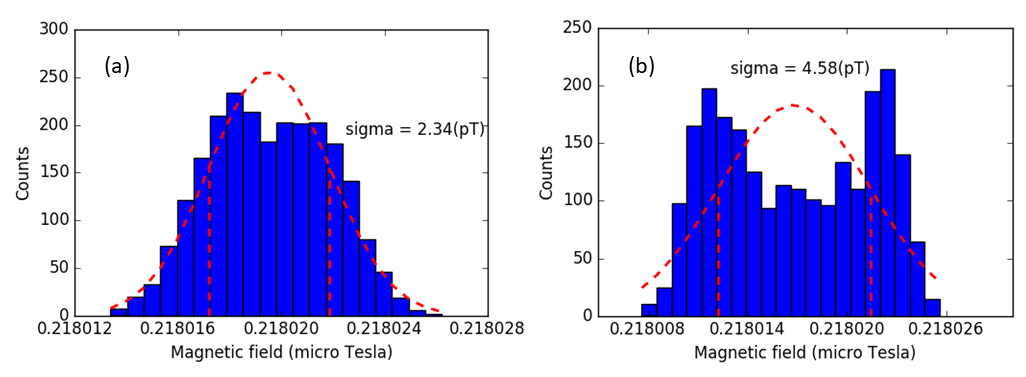
\includegraphics[width=\textwidth]{figures/pump_beam}
  \caption{Magnetic field histograms for different pump beam duty
    cycles (a) 5\% (b) 16\%.  Numbers written on the graph report the
    standard deviation of each distribution.}
    \label{fig:different pump power}
\end{figure}

The histogram of measured magnetic field for two different pump beam
powers is shown in Fig.~\ref{fig:different pump power}. The standard
deviation becomes larger for higher duty cycle while it becomes
narrower for small duty cycle.  It is clear from the plot that the
data points are not statistically distributed.  

It was observed very clearly during these studies that when a pump
beam with a higher duty cycle was used, the FID amplitude increased
until a saturation point.  The data in Fig.~\ref{fig:different pump
  power}(b) are close to this saturation point.  But the problem of
non-statistical behavior is also more apparent.  So it can be
concluded that using higher duty cycle is likely statistically more
robust, revealing new systematic errors in field measurement which led
to the next studies.

\subsection{Reference frequency of lock-in amplifier and precision frequency measurement}

The measurement technique of FID signal was discussed in
Section~\ref{sec:FID}.  In order to capture the FID signal, the
reference frequency of lock-in amplifier is normally set to $\sim
100$~Hz apart from the resonance frequency.  Also the lock-in time
constant was set to 300~$\mu$s.  Technically, this time constant too
loow.  It admits frequency components beyond the reference frequency
which is typically 2000~Hz, if the magnetic field being measured is of
order 0.2~$\mu$T.  Because of the bimodal structure seen in
Figs.~\ref{fig:different probe power} and~\ref{fig:different pump
  power}, we began to suspect that some noise was creeping into the
frequency measurement through the lock-in amplifier.

This led us to increase the lock-in time constant, which in turn led
us to want to reduce the frequency difference between the lock-in
reference frequency and the atoms.

%In this study we kept all other setting fixed only changed the Lock-in
%reference frequency and observed the effect of that on field
%measurement study. The measurement was conducted at $0.2~\mu$T field.
\begin{figure}
  \centering
  \begin{subfigure}[b]{0.47\textwidth}
    \centering
    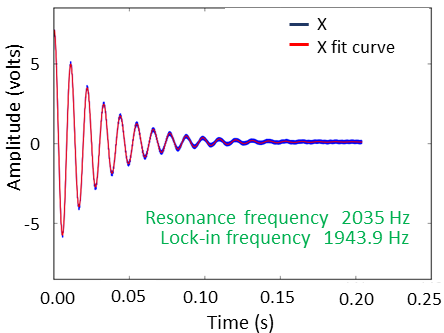
\includegraphics[width=\textwidth]{figures/reference_frequency1}
    \caption{}
    \label{fig:far from resonance}
  \end{subfigure}
  \hfill
  \begin{subfigure}[b]{0.47\textwidth}
    \centering
    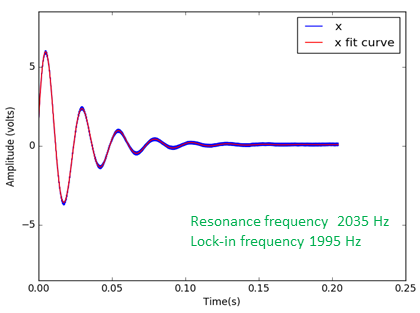
\includegraphics[width=\textwidth]{figures/reference_frequency3}
    \caption{}
    \label{fig: middle range}
  \end{subfigure}
  \begin{subfigure}[b]{0.47\textwidth}
    \centering
    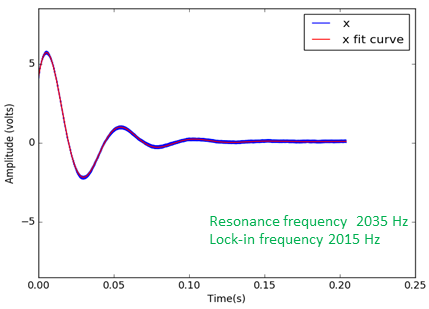
\includegraphics[width=\textwidth]{figures/reference_frequency2}
    \caption{}
    \label{fig:close to resonance}
  \end{subfigure}
  \caption{FID signal for different reference frequency settings of
    the lock-in amplifier, while the true magnetometer resonance
    frequency was roughly 2035~kHz (which was the AOM frequency
    setting) (a) lock-in reference frequency 1943.9~Hz (b) 1995~Hz,
    and (c) 2015 Hz.\label{fig:different reference signal}}
\end{figure}

The FID signal for different reference frequency of lock-in amplifier
is shown in Fig.~\ref{fig:different reference signal}.  The data are
fitted in order to determine the frequency of oscillation.  In this
case the pump power was 60~$\mu$W and the probe power was 30~$\mu$W.
We decided to study these settings in more detail.

\begin{figure}%[h]
\centering
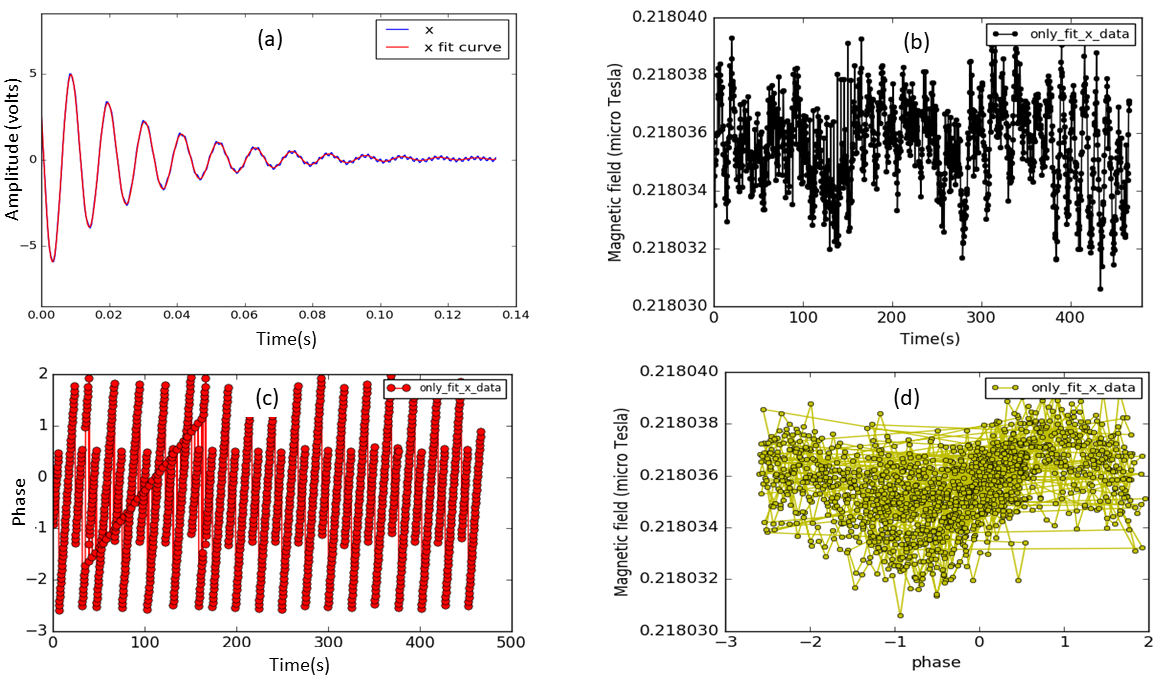
\includegraphics[width=\linewidth]{figures/freq_1943_single_fit_300microsec.png}
\caption{Lock-in reference frequency and time constant are 1943 Hz and
  300~$\mu$s respectively.  Only X data was fitted.  (a) example of an
  FID and individual fit (b) frequency measurement translated to
  magnetic field (c) phase of fit (d) magnetic field
  vs.~phase.\label{fig:freq_1943_single_fit_300_micros}}
\end{figure}

Fig.~\ref{fig:freq_1943_single_fit_300_micros} displays study over
time of the 1943~Hz lock-in amplifier frequency setting.  In the
example FID in Fig.~\ref{fig:freq_1943_single_fit_300_micros}(a) some
high frequency periodic noise can be seen.  In
Fig.~\ref{fig:freq_1943_single_fit_300_micros}(b) some non-statistical
sinusoidal behavior can be seen.  We eventually realized that this was
correlated with the phase determined by the fit.  The phase as a
function of time is shown in
Fig.~\ref{fig:freq_1943_single_fit_300_micros}(c).  The correlation of
field with phase is shown in
Fig~\ref{fig:freq_1943_single_fit_300_micros}(d).  An indication of
correlation between field and phase can be seen here.

Clearly it is possible for the frequency to be pulled by the phase of
the fit, given that the precision of the frequency fit is determined
in part by the number of zero-crossings in the individual FID signals.
The phase could certainly affect the number of zero crossings which
are statistically relevant to the fit.

\begin{figure}%[h]
\centering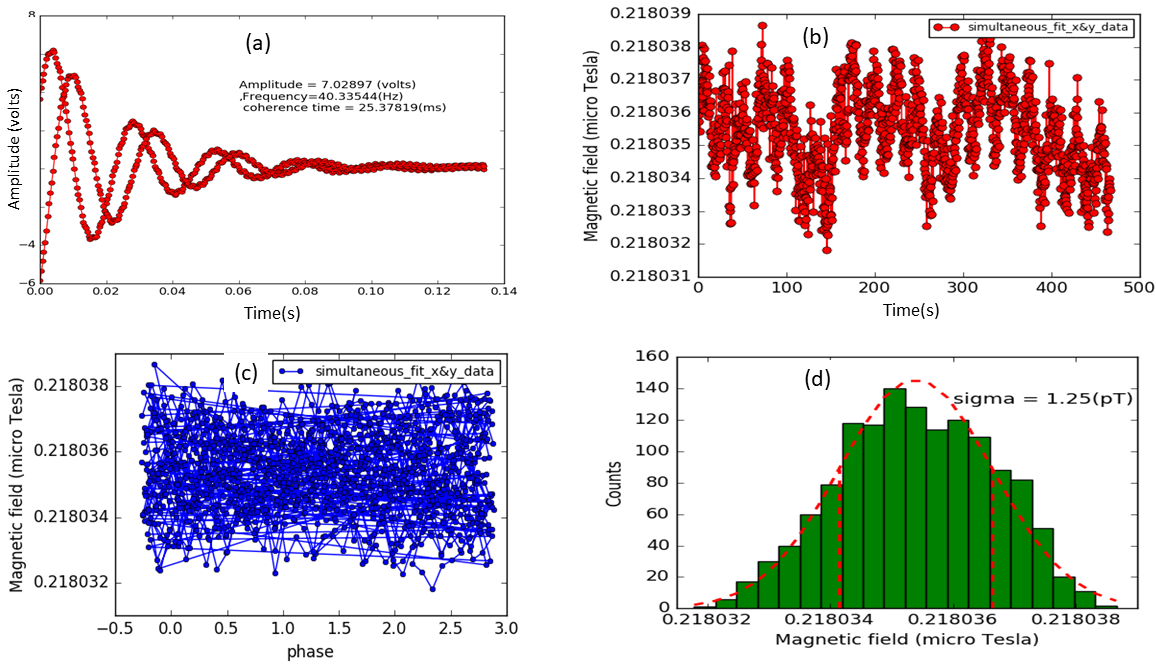
\includegraphics[width=\linewidth]{figures/freq_1943_simultaneous_fit_300microsec_.png}
\caption{Lock-in reference frequency and time constant are 1943 Hz and
  300~$\mu$s respectively.  X and Y data were fitted simultaneously.
  (a) example of an FID and its fit (b) frequency measurement
  translated to magnetic field (c) magnetic field vs.~phase determined
  by fit (d) histogram of field
  measurements.\label{fig:freq_1943_simultaneous_fit_300_micro_sec}}
\end{figure}

We decided to try to reduce the dependence on phase by fitting both
the X and Y signals simultaneously.
Fig.~\ref{fig:freq_1943_simultaneous_fit_300_micro_sec} shows this
study.  From
Fig.~\ref{fig:freq_1943_simultaneous_fit_300_micro_sec}(c), it can be
seen that the correlation of frequency with phase has been reduced
significantly, so that the data look statistical when histogrammed, as
is done in Fig.~\ref{fig:freq_1943_simultaneous_fit_300_micro_sec}(d).
But Fig.~\ref{fig:freq_1943_simultaneous_fit_300_micro_sec}(b) still
clearly shows that there is non-statistical behavior in the frequency
(field) measurements.  We though this might yet be due to the periodic
high-frequency noise seen if
Fig.~\ref{fig:freq_1943_simultaneous_fit_300_micro_sec}(a).  Based on
this we decided to increase the lock-in time constant, and tried
increasing the lock-in reference frequency to have more flexibility to
change the time-constant.

\begin{figure}%[h]
\centering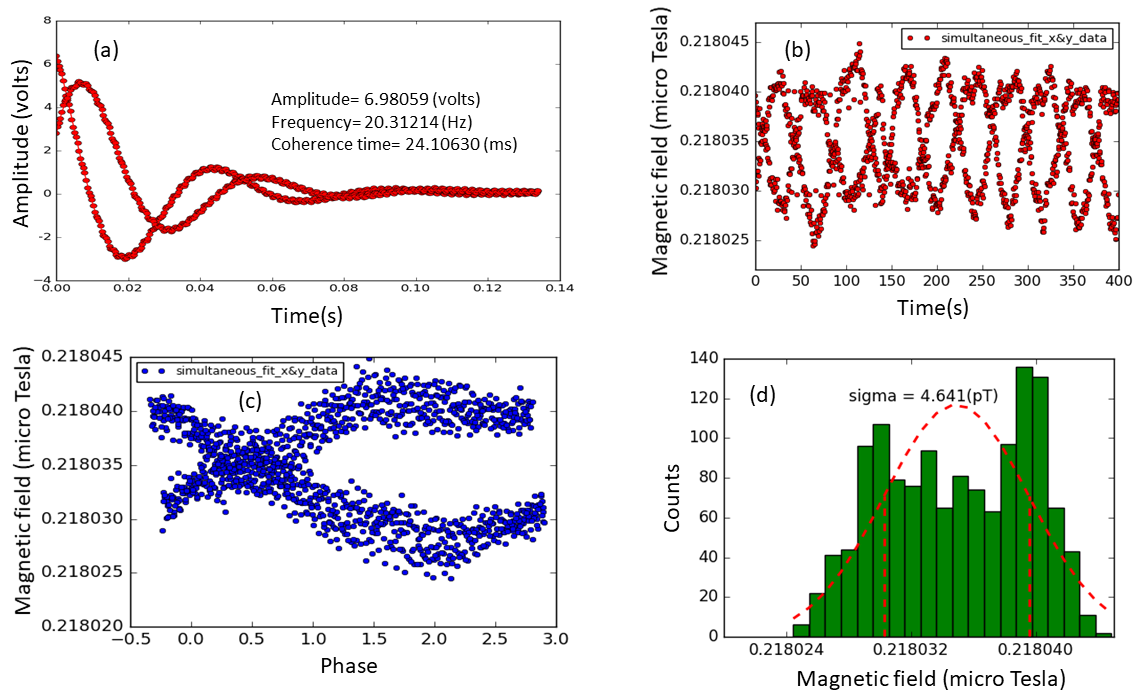
\includegraphics[width=\linewidth]{figures/freq_2015_simultaneous_fit_300microsec.png}
\caption{Lock-in reference frequency and time constant are 2015~Hz and
  300~$\mu$s respectively.  X and Y data were fitted simultaneously.
  (a) example of an FID and its fit (b) frequency measurement
  translated to magnetic field (c) magnetic field vs.~phase determined
  by fit (d) histogram of field
  measurements.\label{fig:freq_2015_simultaneous_fit_300_micros}}
\end{figure}

In Fig.~\ref{fig:freq_2015_simultaneous_fit_300_micros}, the lock-in
reference frequency has been changed to 2015~Hz, without yet changing
the lock-in time constant.  The interesting feature here is that,
although the X and Y data are fitted simultaneously, there is a very
clear phase dependence to the field measurements.  The ``best'' choice
of phase appears to be about 0.5~radians.  It is not unexpected to
have such a phase dependence, given that there are so few
zero-crossings in the FID signal that can be used to constrain the
frequency.

\begin{figure}%[h]
\centering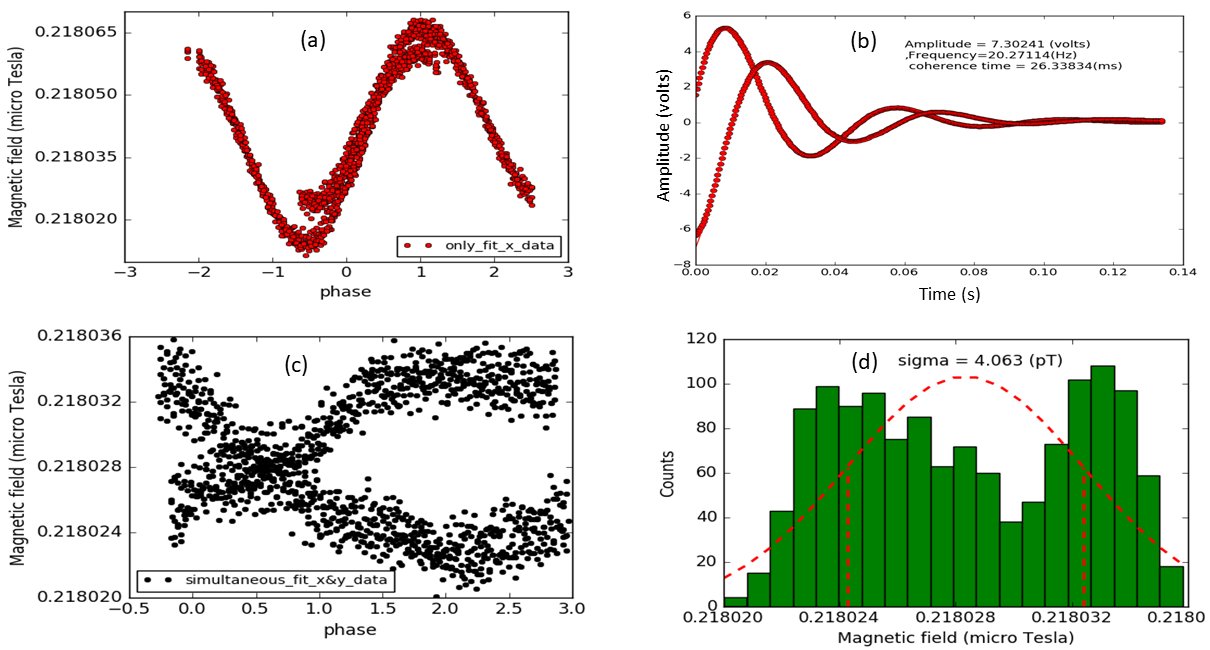
\includegraphics[width=\linewidth]{figures/freq_2015_simultaneous_fit_1ms.png}
\caption{Lock-in reference frequency and time constant are 2015~Hz and
  1~ms respectively.  (a) frequency measurement determined by fit of X
  data only as a function of the phase also determined by that fit (b)
  example of an FID and its fit, where both X and Y data has been
  fitted simultaneously (c) magnetic field vs.~phase determined by the
  simultaneously fitted X and Y data (d) histogram of field
  measurements arising from the simultaneous fit of the X and Y
  data.\label{fig:freq_2015_1ms}}
\end{figure}

In Fig.~\ref{fig:freq_2015_1ms}, the lock-in reference frequency of
2015~Hz has been retained, but the lock-in time constant has now been
increased to 1~ms.  The same large phase dependence can be seen.
Fig.~\ref{fig:freq_2015_1ms}(a) additionally shows the phase
dependence of the fit to the X data only, which is even larger.  Aside
from the strong phase dependence, the data do appaear to be
statistical in nature.

\begin{figure}%[h]
\centering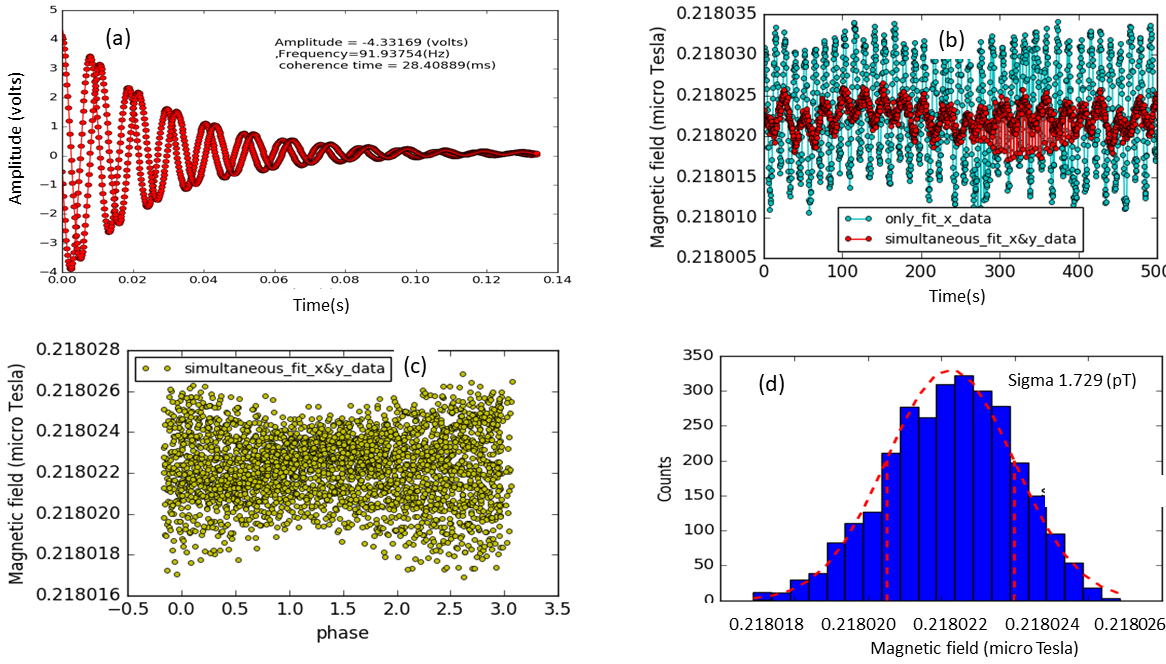
\includegraphics[width=\linewidth]{figures/freq_1943_simultaneous_fit_1ms.png}
\caption{Lock-in reference frequency and time constant are 1943~Hz and
  1~ms respectively (a) example of an FID and its simultaneous fit to
  the X and Y data (b) frequency measurement translated to magnetic
  field, in red are shown the results of the simultaneous fit to the X
  and Y data, in cyan are the results of the fit to the X data only
  (c) magnetic field vs.~phase determined by the simultaneous fit to
  the X and Y data (d) histogram of field measurements for the
  simultaneously fitted X and Y
  data.\label{fig:freq_1943_simultaneous_fit_1ms}}
\end{figure}

In Fig.~\ref{fig:freq_1943_simultaneous_fit_1ms} the lock-in reference
frequency has been set to 1943 Hz and the lock-in time constant to
1~ms.  Compared with the 300~$\mu$s settings which were shown in
Figs.~\ref{fig:freq_1943_single_fit_300_micros}
and~\ref{fig:freq_1943_simultaneous_fit_300_micro_sec}, the phase
dependence has been accentuated by the longer lock-in time constant.
Another feature is that the amplitude of the fitted data has been
reduced, seen particularly in
Fig.~\ref{fig:freq_1943_simultaneous_fit_1ms}(a).

The main conclusion of these studies was that the frequency fitting
procedure is quite sensitive to the lock-in time constant and
frequency settings, which may induce errors if not adjusted carefully.
These could give rise to additional systematic errors.  This would be
one of the main topics for further study in order to push the
precision of the magnetometer to its limits.  Generally these effects
manifest themselves as fairly obvious nonstatistical behaviors in the
data either as a function of time or when histogramming the field
measurements.  They also tend to become an issue with frequency
measurements of precision below 1~Hz are made on each individual FID
measurement.

It is also worth noting that all the above studies were done for a
considerable larger probe power than the optimal low value.  As a
consequence the coherence times are rather short compared to the
values used for most other studies in this thesis.  The frequency
measurements of the other studies are less affected by these phase
effects as a result.


\section{Tilted field measurements} 
\label{sec:tilted-results}

 %\begin{figure}
    %\centering
    %\begin{subfigure}[b]{0.45\textwidth}
       % \centering
       % %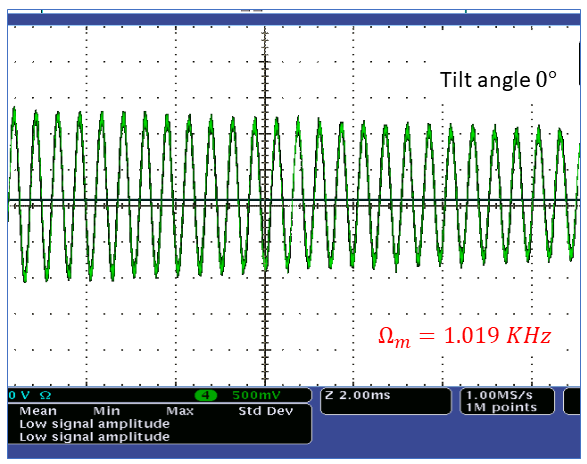
\includegraphics[widt%h=\textwidth,trim={0cm 0.5cm 0cm 0cm},clip]{figures/tilt1.png}
        %\caption{}
        %\label{fig:tilt_0_degree}
    %\end{subfigure}
   % \caption{Optical rotation as a function of time at $\Omega_L$ in the yz plane for different tilt angle.\label{fig:optical-rotation-different-angle}}
%\end{figure}

%\begin{figure}
%  \centering
%  %trim={<left> <lower> <right> <upper>}
%  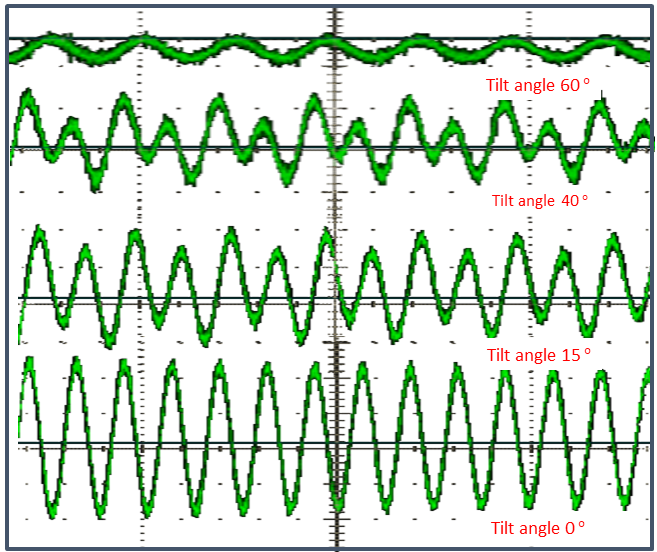
\includegraphics[width=0.8\textwidth]{figures/tilted_field_scope_trace.png}
%  \caption{Differential photodiode signal as a function of time zoomed
%    in on the FID measurement region.  The time base is 2~ms per
%    division. 
%
%at $\Omega_L$ in the
%    yz plane for different tilt
%    angle.\label{fig:optical-rotation-different-angle}}
%\end{figure}

%In this Rb NMOR magnetometry setup the rubidium atoms interacted with
%a $z$-directed laser light beam which is linearly polarized along the
%y axis. In the FID NMOR technique, the magnetic field is generally
%directed along the light propagation direction and the resonance
%occurs at $2\Omega_L$.  This effect can be explained by considering
%that the polarization returns to its original state after a
%$180\degree$ rotation because of the two-fold symmetry of the
%optically pumped state. As a result, the optical rotation induced by
%the rotating linear dichroism is periodic at twice the Larmor
%frequency.

%We have observed that Resonances in nonlinear magneto-optical rotation with amplitude modulated light by tilting the magnetic field at angles away from the direction of light propagation while operating the Rb magnetometer in FID mode. When the field is tilted in the plane perpendicular to the light polarization direction an resonance appears at $2\Omega_L$. In this case no additional resonance appears for modulation frequency $\Omega_L$. The amplitude of the FID NMOR signal decreases with increasing tilt angle. 

%However, We also observed that by tilting the field direction toward the light polarization direction a new resonance occurs at $\Omega_L$ along with the main resonance at $2\Omega_L$. The resonance signal recorded at $\Omega_L$ contains two frequency components.

In Section~\ref{sec:ch4_tilted_field} we described magnetometer
operations for tilted field, where we did not use the lock-in
amplifier.  We showed an example where the field was tilted in the
$yz$-plane which is defined by the laser propagation direction ($z$)
and the $y$-coil direction.

When the pump beam is modulated at $\Omega_m\approx \Omega_L$, the FID
signal shows two frequency components: one near $2\Omega_L$ and one
near $\Omega_L$.  The amplitude of these frequency components is
sensitive to the tilt angle. One of them is the FFT of FID signal and
the other one is the fit FID signal using
\begin{equation}
  X(t)=A_1e^{-t/\tau_1}\sin(\omega_1t+\phi_1)+A_2e^{-t/\tau_2}\sin(\omega_2t+\phi_2)+C
\label{eq:two_sinewave}
\end{equation}
where $X(t)$ is the differential photodiode signal as a function of
time, and $A_1$, $A_2$, $\omega_1$, $\omega_2$, $\phi_1$, $\phi_2$,
$\tau_1$, and $\tau_2$ are fit parameters.  A 10th order Infinite
Impulse Response (IIR) Butterworth filter was used at times to reduce
background noise from the signal \cite{key}.

\begin{figure}%[h]
\centering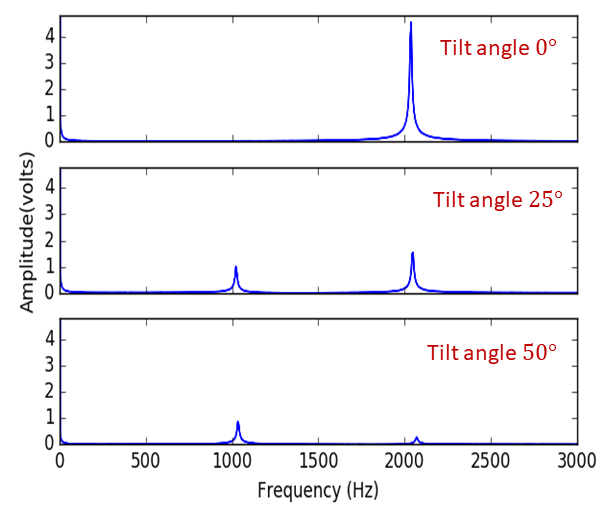
\includegraphics[width=0.7\linewidth]{figures/fft_amp.png}
\caption{FFT of FID signal in the presence of transverse field after
  amplitude modulation at frequency $\Omega_m=1019$~Hz.  The topmost
  figure shows when the field is oriented along the $z$-axis (the axis
  of the laser beam path).  The middle figure shows when the field has
  been oriented at a 25\degree angle relative to the $z$-direction in
  the $yz$-plane.  The bottom figure shows when the field has been
  oriented at a 50\degree angle relative to the $z$-direction in the
  $yz$-plane.\label{fig:fft-amplitude}}
\end{figure}

Fig.~\ref{fig:fft-amplitude} display the FFT of resonance signal for
three different tilt angles of $0\degree$, $25\degree$ and $50\degree$
in the $yz$-plane. It can be seen from the plot that at $0\degree$
tilt angle there is only one frequency component while for others two
peaks correspond to two frequency components.

\begin{figure}
  \centering
  \begin{subfigure}[b]{0.49\textwidth}
    \centering
    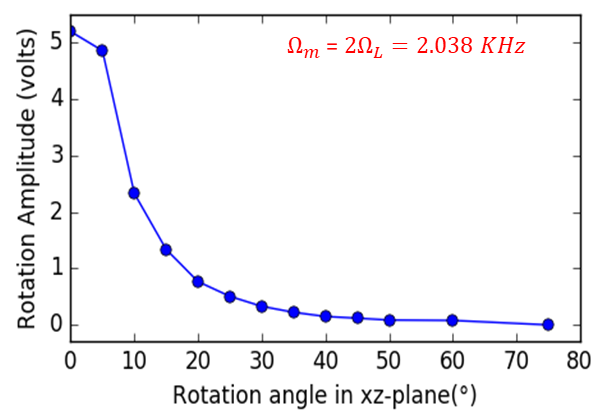
\includegraphics[width=\textwidth]{figures/tilt_x_larmor.png}
    \caption{}
    \label{fig:y equals x}
  \end{subfigure}
  \hfill
  \begin{subfigure}[b]{0.49\textwidth}
    \centering
    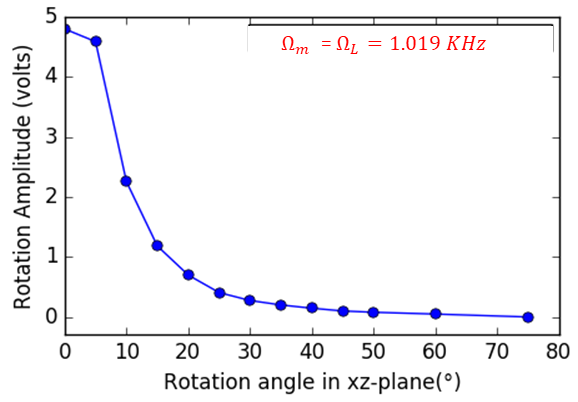
\includegraphics[width=\textwidth]{figures/tilt_x_2larmor.png}
    \caption{}
    \label{fig:three sin x}
  \end{subfigure}
  \caption{The amplitude of the FID NMOR signals seen near $2\Omega_L$
    as a function of tilt angle recorded at (a) $\Omega_m\approx
    2\Omega_L$ and (b) $\Omega_m\approx 2\Omega_L$ vs.~the tilt angle
    of the magnetic field in the plane defined by the
    light-polarization and light propagation vectors ($xz$-plane).
    The amplitude of the FID signal at $\Omega_L$ was
    small.\label{fig:tilted-wrong}}
\end{figure}
Fig.~\ref{fig:tilted-wrong} shows the amplitude of the FID signal for
the magnetic field tilted in the $xz$ plane (which we assume means out
of the polarization plane) at various angles to the light propagation
direction at modulation frequencies $\Omega_m=2\Omega_L$ and
$\Omega_L$. It can be seen from the figure that the amplitude of the
FID signal decreases with increasing tilt angle for both modulation
frequencies.  It is dominated by a single frequency component near
$2\Omega_L$.

\begin{figure}
  \centering
  \begin{subfigure}[b]{0.49\textwidth}
    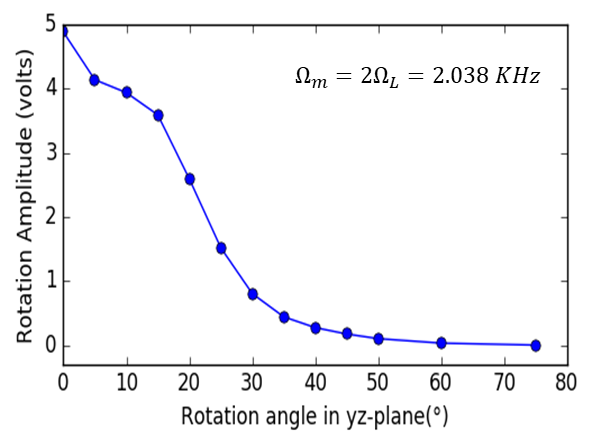
\includegraphics[width=\textwidth]{figures/tilt_y_larmor.png}
    \caption{}
    \label{fig:tilt_y}
  \end{subfigure}
  \hfill
  \begin{subfigure}[b]{0.49\textwidth}
    \centering
    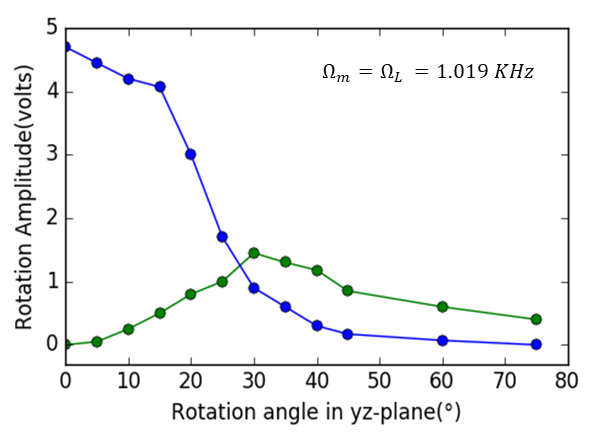
\includegraphics[width=\textwidth]{figures/tilt_y_2larmor.png}
    \caption{}
    \label{fig:tilt_x}
  \end{subfigure}
  \caption{The amplitude of the FID NMOR signals as a function of tilt
    angle for pumping frequencies near (a) $\Omega_m=2\Omega_L$ and
    (b) $\Omega_L$ vs. the tilt angle of the magnetic field in the
    plane defined by the light-polarization and light propagation
    vectors ($yz$-plane). For the data in (a), a single frequency
    component at $2\Omega_L$ tended to dominate, and the amplitude of
    this signal is shown.  For the data in (b), two frequency
    components in the FID signal were seen.  The amplitude of the
    signal at $2\Omega_L$ is shown in blue and the amplitude of the
    signal at $\Omega_L$ is shown in
    green.\label{fig:something-tilted}}
\end{figure}

Fig.~\ref{fig:something-tilted}(a) indicates the signal amplitude
vs. different tilt angle at $\Omega_m=2\Omega_L$ . The amplitude of
fitted FID signal at $2\Omega_L$ decreases as the angle between
magnetic field and the light propagation direction increases.

Fig.~\ref{fig:something-tilted}(b) shows the FID amplitudes for a
pumping frequency $\Omega_m=\Omega_L$. The FID at $2\Omega_L$
decreases with increasing tilt angle in $yz$-plane, while the FID
amplitude at $\Omega_L$ increases till $30\degree$ and after that the
amplitude starts to decrease, but still dominates over the signal at
$2\Omega_L$. For both cases (Fig.~\ref{fig:tilted-wrong} and
Fig.~\ref{fig:something-tilted}) the signal amplitude has been
extracted as a fit parameter when data was fitted to the fit function
\ref{eq:two_sinewave}

\begin{figure}%[h]
\centering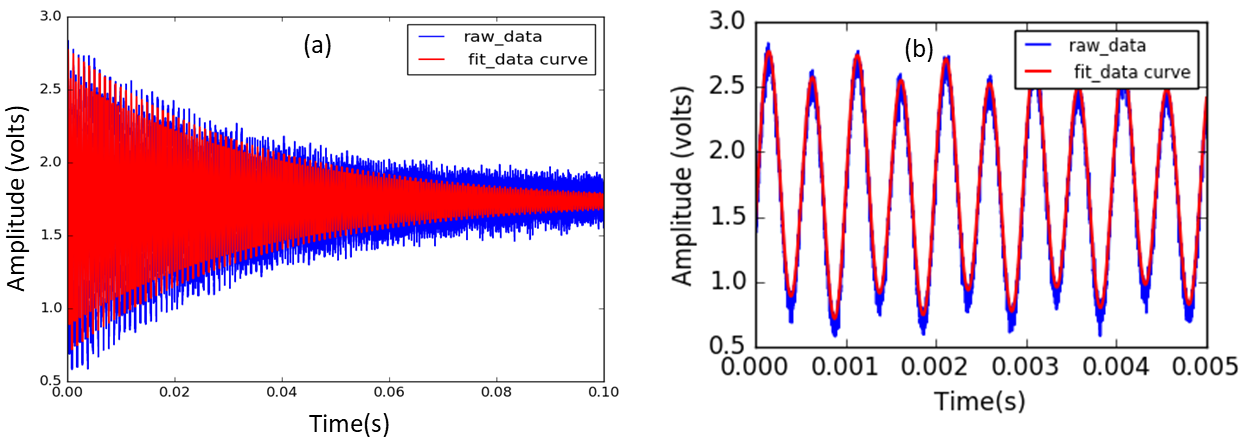
\includegraphics[width=\linewidth]{figures/fitted_data_tilted_field.png}
\caption{Fitted FID signal using Eq. \ref{eq:two_sinewave}. (b) The
  zoomed version of (a). The blue line indicates raw data while the
  red one indicates fitted curve.\label{fig:ex1}}
\end{figure}

\begin{figure}%[h]
\centering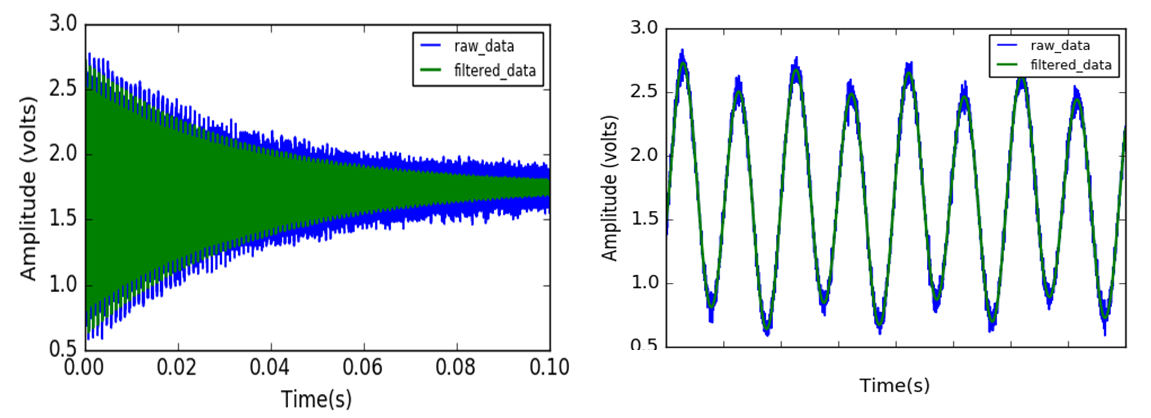
\includegraphics[width=\linewidth]{figures/filtered_data.png}
\caption{(a) Raw and filtered FID signal. (b) zoomed version of
  (a).\label{fig:ex2}}
\end{figure}

Figs.~\ref{fig:ex1} and~\ref{fig:ex2} show examples of the quality of
fit for unfiltered data, and the quality of the data after filtering
respectively.

The conclusion is that pumping at $\Omega_m=\Omega_L$ followed by
detection of the FID at frequencies $2\Omega_L$ and $\Omega_L$ would
allow detection of the field and its angle in the $yz$-plane
simultaneously.  While this is consistent with previous work in the
literature, it represents the first use of FID measurements to make
the deduction.

In the future, further improvements to the calibration of the
measurements would be made in order to see whether how small a tilt
angle could be measured.  In the nEDM experiment, the field magnitude
is 1~$\mu$T, and if this magnetometer could sense transverse fields at
the 1~nT level, it would be a new application of such magnetometry
techniques.
